% Copyright (C)  2015  Philipp Hacker.
% Permission is granted to copy, distribute and/or modify this document
% under the terms of the GNU Free Documentation License, Version 1.3
% or any later version published by the Free Software Foundation;
% with no Invariant Sections, no Front-Cover Texts, and no Back-Cover Texts.
% The lincense itself can be found at <https://www.gnu.org/licenses/fdl-1.3>.

\documentclass[numbers=noenddot,a4paper]{scrartcl}

\usepackage[greek,ngerman]{babel}
\usepackage[T1]{fontenc}
%\usepackage[applemac]{inputenc}
\usepackage[utf8]{inputenc}
\usepackage{fullpage}
\usepackage{scrpage2}
\usepackage{libertine}
%\usepackage{braket}
\usepackage{ziffer}
\usepackage{graphicx}
\usepackage{units}
\usepackage[infoshow]{tabularx}
\usepackage[all]{xy}
\usepackage{amsmath}
\usepackage{amssymb}
\usepackage{wrapfig}
\usepackage{upgreek}
\usepackage{esint}
\usepackage{float}
\usepackage[font=small,labelfont=bf]{caption}
\usepackage{subcaption}
\usepackage{lscape}
\usepackage[backref=page]{hyperref}
\usepackage{csquotes}
\usepackage[printonlyused,withpage,footnote]{acronym}

\renewcommand{\thefigure}{Abb. \arabic{figure}}
%\renewcommand{\bflabel}[1]{\normalfont{\normalsize{#1}}\hfill}

%\captionsetup[wrapfigure]{name=}
\captionsetup[figure]{name=}

\newcommand{\nummat}[1]{\left[\text{#1}\right]}
\newcommand{\num}[1]{$\left[\text{#1}\right]$}
\newcommand{\degree}{^\circ}
\newcommand{\diff}{\textnormal{d}}
\newcommand{\tenpo}[1]{ 10^{#1}}
\newcommand{\greek}[1]{\greektext#1\latintext}
\newcommand{\ix}[1]{_\text{#1}}
\newcommand{\imag}{\mathbf{i}}
\newcommand{\tilt}[1]{\textit{#1}}
\newcommand{\grad}[1]{\textit{grad}\left(#1\right)}
\newcommand{\divergenz}[1]{\textit{div}\left(#1\right)}
\newcommand{\euler}{\mathnormal{e}}
\newcommand{\fett}[1]{\textbf{#1}}
\newcommand{\einnup}{\hspace{0.2cm}}
\newcommand{\einnum}{\hspace{-0.2cm}}
\newcommand{\zentriert}[1]{\begin{center}#1\end{center}}

\title{Bachelor-Arbeit zum Thema \enquote{Modenanregung in \tilt{Yukawa}-Bällen}} %TODO Name
\author{Philipp Hacker} %TODO Author
\date{\today}

\setcounter{section}{-1}

\begin{document}

	\maketitle

	\begin{center}

		Institut für Physik\\
		mathematisch-naturwissenschaftliche Fakultät\\
		Universität Greifswald

	\end{center}
	
	\vspace{0.5cm}

	\begin{figure}[H]
			\centering
			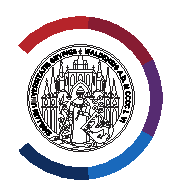
\includegraphics[width=0.35\textwidth]{figs/unilogo_NEU_schwarz.eps}
	\end{figure}

	\vspace{0.5cm}

	\begin{center}

			\hspace{-0.55cm} Erst-Gutachter: Prof. Dr. André Melzer \\ \vspace{0.25cm} %TODO Name Erst-Gutachter

			Zweit-Gutachter: Prof. Dr. Lutz Schweikhard \\ \vspace{0.25cm} %TODO Name Zweit-Gutachter

			Bearbeitungszeitraum: 01.03.2015 bis 12.07.2015 \\ \vspace{0.25cm} %TODO Bearbeitungszeitraum

%		\begin{table}[h]
%			\centering
%			Note (Erst-Gutachter): %TODO Gute Note erhalten :)
%			\begin{tabularx}{1.5cm}{|X|}
%				\hline \\ \\
%				\hline
%			\end{tabularx}
%			
%			\centering
%			\hspace{-0.42cm} Note (Zweit-Gutachter): %TODO Gute Note erhalten :)
%			\begin{tabularx}{1.5cm}{|X|}
%				\hline \\ \\
%				\hline
%			\end{tabularx}
%			
%		\end{table}

	\end{center}

	\thispagestyle{empty}

	\newpage

	\tableofcontents

	\newpage

	\section{Motivation}\label{sec:einleitung}

	\newpage

	\section{Physikalische Grundlagen}\label{sec:physg}

		In diesem ersten Abschnitt soll der Hintergrund f\"ur den sich anschlie{\ss}nenden Versuch gegeben werden. Dabei wird einerseits auf grundlegendes aus der Plasmaphysik sowie komplexer Plasmen eingegangen, andererseits aber auch auf die theoretischen Modelle, welche essentiell f\"ur das Verst\"andnis der Ph\"anomene dieses Experiments sind.

		\subsection{Kapazitiv gekoppelte Radiofrequenz-Plasmen} \label{sub:kaprfplasm}

			Der in diesem Versuch genutzte Aufbau entspricht dem eines kapazitiv gekoppelten Niederdruck-Radiofreuquenz-Plasmas.\\
			Ein Plasma ist ein quasineutrales Gas aus freien Ladungsträgern und, dem Ionisierungsgrad der Entladung entsprechend, neutralen Atomen oder Molekülen. Die Spezies der Ladungen sind im allgemeinen Elektronen und Ionen, wobei der Begriff quasineutral die Bedingung $n\ix{e}=n\ix{I}$ der Dichten auf einer speziellen Längenskala fordert (siehe unten). Für ein Plasma gibt es verschiedene physikalischen Kenngrößen, welche in Tabelle \ref{tab:kenngroessen} inklusive ihrer Bedeutungen einmal zusammengefasst wurden.\\
			Befindet sich ein Fremdteilchen, ein Festkörper oder eine weitere Ladungsträgerspezies in der Entladung, so spricht man von komplexen Plasmen. Für das Experiment dieser Arbeit ist dies der Fall, da hierbei in das Plasma homogene Melamin-Formaldehyd-Partikel in der Größenordnung einiger $\unit{\mu m}$ eingebracht werden. Diese erfahren, in Abhängigkeit der Parameter, verschiedenste Wechselwirkungen mit den Entladungsspezies und externen Feldern.

				\begin{table}[H]
					\centering
						\begin{tabular}{m{0.3\textwidth}|m{0.3\textwidth}|m{0.3\textwidth}}
							Größe & Zusammenhang & Bedeutung \\ 
							\hline  Debye-Länge & $\lambda\ix{D,j}^2=\frac{\varepsilon\ix{0}k\ix{B}T\ix{j}}{n\ix{j}e^2}$
							\newline
							$\lambda\ix{D}^2=\left(\lambda\ix{D,e}^{-2}+\lambda\ix{D,I}^{-2}\right)^{-1}$ & die Distanz um eine Probeladung, ab welcher die Quasineutralität gilt und gleichzeitig, wann die Ladung vollständig abgeschirmt ist \\ 

							\hline Plasmafrequenz & $\omega\ix{P,j}^2=\frac{n\ix{j}e^2}{\varepsilon\ix{0}m\ix{j}}=\frac{v\ix{th,j}}{\lambda\ix{D,j}}=\frac{1}{\tau\ix{j}}$ & obere Grenze der Zeitskala für die Wechselwirkung mit externen Kräften bzw. Feldern; Inverse der Abschirmungszeit \\ 

							\hline thermisches Geschwindigkeit & $v\ix{th,j}^2=\frac{k\ix{B}T\ix{j}}{m\ix{j}}$ & mittlere Geschwindigkeit aus der Definition der kinetischen Gastheorie \\ 

							\hline mittlerer Teilchenabstand & $\overline{b}=\frac{\hbar}{m\ix{j}v\ix{th,j}}$ & gemittelter Teilchenabstand, entspricht thermischer \mbox{\tilt{de-Broglie}-Wellenlänge} \\ 

							\hline Yukawa-Potential & $\Phi=\frac{Q}{4\pi\varepsilon|\vec{r}|}\euler^{-\frac{|\vec{r}|}{\lambda\ix{D}}}$ & elektrostatisches Wechselwirkungspotential einer Probeladung $Q$ in einem Plasma (Vergleich Pionen-Austausch) \\

							\hline

						\end{tabular}
					\caption{Plasmaphysikalische Kenngrößen. Der Index $j$ bestimmt die Ladungsträgerspezies mit den entsprechenden Massen und Ladungen.}
					\label{tab:kenngroessen}
				\end{table}

			Wie bereits erwähnt greift dieses Experiment auf die Erzeugung einer Gasentladung zurück. Hierbei ist der Versuch wie ein horizontal ausgerichteter, paralleler Plattenkondensator angeordnet (siehe \ref{img:ungleichesplasma}), wobei das Dielektrikum das Plasma sei, die untere Elektrode mit einem Signal im $\unit{MHz}$-Bereich betrieben wird und die andere auf Massepotential liegt. Das elektrische Feld resultiert hierbei aus den Oberflächenladungen der Elektroden, wobei mit unterschiedlichen \tilt{rf}-Signalen (\tilt{radio frequency}) auch verschiedene Betriebsregime realisiert, e.g. Ladungsträger erzeugt bzw. vernichtet werden.\\
			Die \tilt{rf}-Spannung sorgt weiterhin für die nötige Homogenität des Plasmas, da aufgrund dessen (wie im $\gamma$-Regime) ein Verschiebungsstrom zwischen Entladungsvolumen und Elektrode fließt (siehe Abschn. \ref{subsub:self-bias}) und damit die Kontaktierung dieser sehr isotrop gestaltet. In Aufbauten, in welchen die Flächen der Elektroden nicht gleich sind, fließt wegen der unterschiedlichen Potentialverläufe in den Randschichten (siehe Abschn. \ref{sub:rand}) zusätzlich eine Gleichspannung, die sogenannte \tilt{self-bias} - siehe Abschn. \ref{subsub:self-bias}. Das ist insbesondere der Fall für das Experiment dieser Arbeit, da hier die gesamte Kammer als Elektrode zur Masse dient und die andere entsprechend kapazitiv an die Erregung gekoppelt ist.

				\subsubsection{Verschiebungsstrom} \label{subsub:verschieb}

					\begin{wrapfigure}{r}{0.4\textwidth}
						\centering
						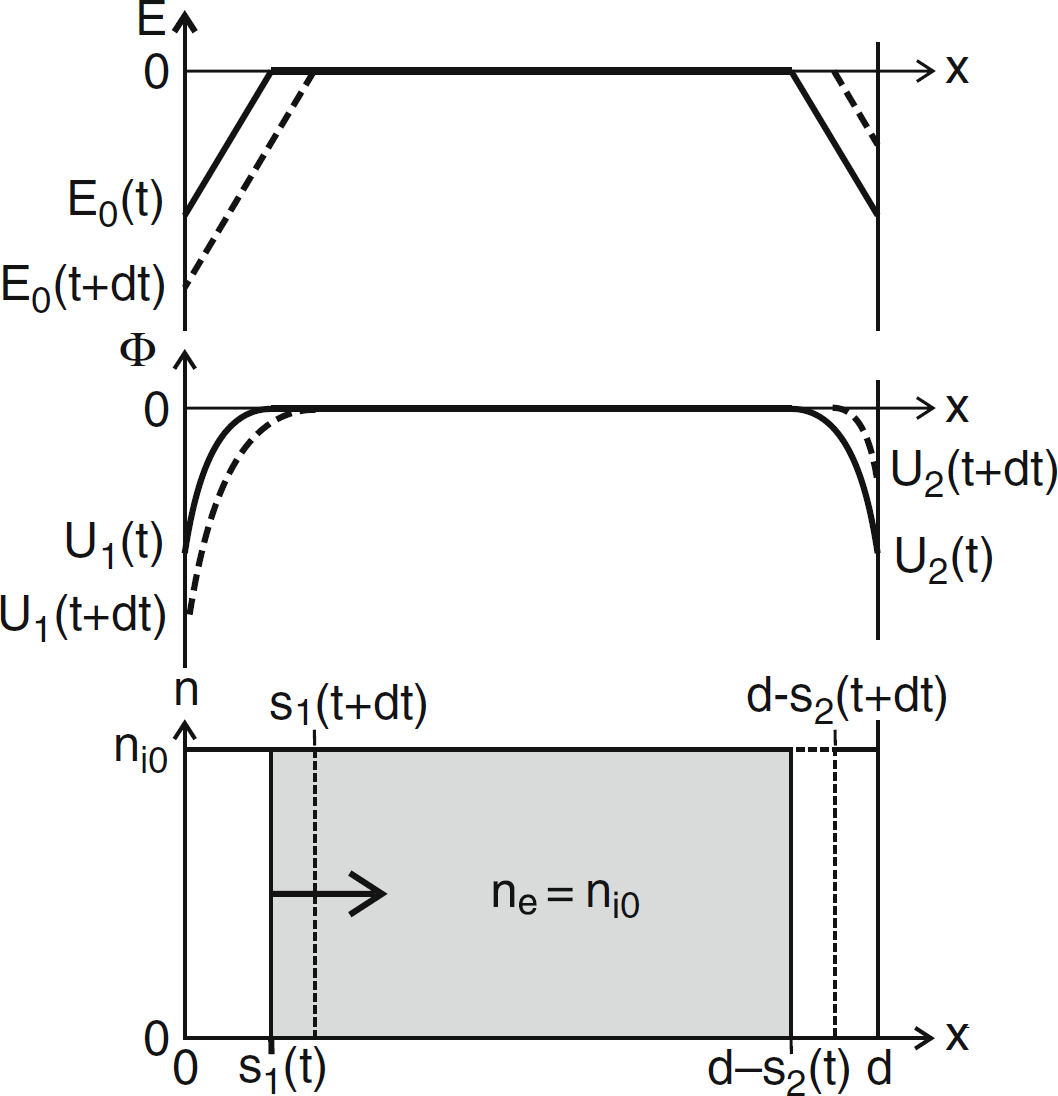
\includegraphics[width=0.47\textwidth,height=0.54\textwidth]{figs/verschiebpiel.png}
						\caption{Verlauf der Dichten, des Elektrischen Feldes und des zug. Potentials (eindimensional) in einer Entladung mit zwei gegenüberliegenden Randschichten (nach \cite{Piel10}).}
						\label{img:verschieb}
					\end{wrapfigure}

				Die Elektronen eines Plasmas über einer \tilt{rf}-getriebenen Elektrode können, aufgrund ihrer Beweglichkeit und hohen Plasmafrequenz $\omega\ix{P,e}$ der Anregung problemlos folgen. Die Ionen sollen in diesem Fall als stationär betrachtet werden, da $\omega\ix{P,I}\ll\omega\ix{P,e}\,$. Nimmt man an, dass die Randschicht der Dicke $a$ frei von Elektronen ist (siehe Abschn. \ref{sub:rand}) und die Ionendichte dort konstant $n\ix{0,I}$ ist, so folgt für das elektrische Feld der positiven Raumladungszone an der Kammerwand $E\ix{0}=-en\ix{0,I}a/\varepsilon\ix{0}\,\,$ - siehe \ref{img:verschieb}. Lädt sich die Entladungsbegrenzung nun stärker negativ auf, so dehnt sich die Randschicht als Folge dessen aus und wandert dabei mit der Geschwindigkeit $v=\diff s\ix{1}/\diff t$ in das Plasmavolumen hinein. Dies führt zum bereits erwähnten Verschiebungstrom in der Randschicht $j\ix{V}=-en\ix{0,I}v$, welcher zusammen mit dem Strom der, aus der Schicht "`verdrängten"' Elektronen $j\ix{L}=-en\ix{0,I}v$ die Kontinuität im Plasma erhält.\\
				Da im Hauptvolumen der Entladung die Quasineutralität erhalten ist, dh. $n\ix{e}=n\ix{0,I}$, müssen die zusätzlichen Elektronen aus der pos. Ladungszone in $x\in\left[0,s\ix{1}+\diff s\ix{1}\right]$ in den Teil des Plasmas, in welchem zu diesem Zeitpunkt die Randschicht schrumpft und $\diff s\ix{1}=-\diff s\ix{2}$ gilt. Daraus folgt wiederum, dass die Randschichten eines harmonisch getriebenen Plasmas sinusoidal um eine Gleichgewichtsdicke $s\ix{0}$ schwingen und während einer jeden Schwingung einmal vollständig verschwinden, e.g. $s\ix{1/2,max}=s\ix{0}\,$.  Letztendlich ergibt sich daraus ein Spannungsabfall über das Plasma aus den Potentialdifferenzen der Randschichten $U\ix{1/2}$:

					\begin{align}
						\Delta U=U\ix{1}-U\ix{2}=-\frac{2en\ix{0,I}s\ix{0}}{\varepsilon\ix{0}}\exp\left(\imag\omega t\right)\,\,.
					\end{align}

				\subsubsection{\tilt{self-bias}}  \label{subsub:self-bias}

						\begin{figure}
							\centering
							\begin{subfigure}[b]{0.48\textwidth}
								\centering
								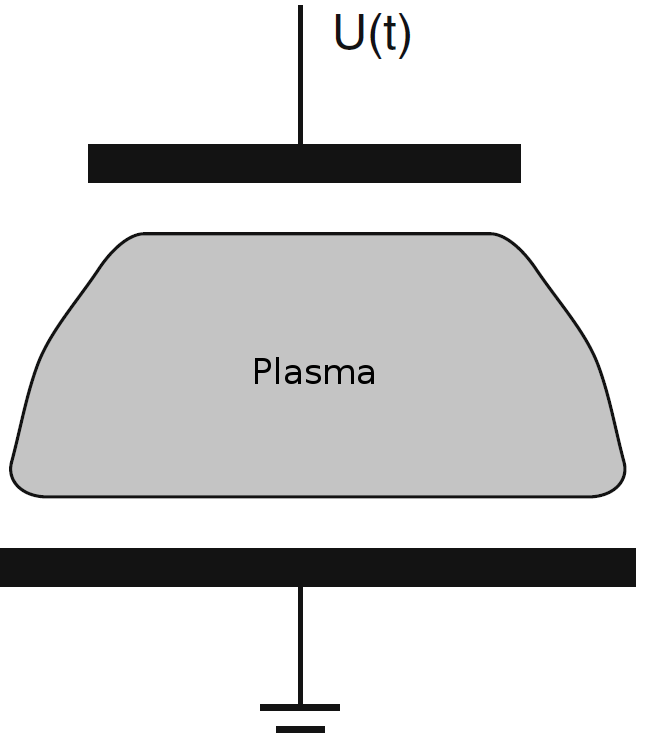
\includegraphics[width=0.7\textwidth,height=0.8\textwidth]{figs/schaltbildselfbiaspiel1.png}
								\caption{}
								\label{img:ungleichesplasma}
							\end{subfigure}
							\begin{subfigure}[b]{0.48\textwidth}
								\centering
								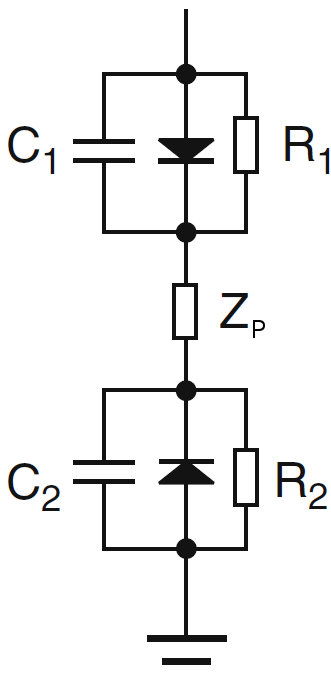
\includegraphics[width=0.4\textwidth,height=0.8\textwidth]{figs/schaltbildselfbiaspiel2.png}
								\caption{}
								\label{img:ersatzschaltbild}
							\end{subfigure}
							\caption{\fett{(a)}:Schema eines Plasmas mit ungleichen Elektrodenflächen. Die obere ist hierbei kleiner und gleichzeitig mit dem \tilt{rf}-Signal betrieben. \fett{(b)}:Ersatzschaltbild einer Entladung mit der \tilt{bulk}-Impedanz $Z\ix{P}$ (Hauptvolumen) und den Randschichten: eine Diode als Symbol für den "`Elektronenfluss"' aus der Schicht hinaus, der Widerstand $R\ix{j}$ als Ionenstrom und die Kapazität $C\ix{j}$ der pos. Raumladungszone (nach \cite{Piel10}).}
						\end{figure}

					Einem Plasma kann man eine, für \tilt{rf}-Spannungen der Frequenz $\omega$ nicht verschwindende Impedanz $Z\ix{P}$ zuordnen. Für das Entladungsvolumen der Permittivität $\varepsilon\ix{P}$, der Kapazität $C\ix{P}$ auf der Querschnittsfläche $A$ und Dicke $b$, in welcher die freien Elektronen mit der Frequenz $\nu\ix{e,N}$ mit den Neutralgasatomen stoßen, gilt:

					\begin{align}
					\varepsilon\ix{P}=1-&\frac{\omega\ix{P,e}^2}{\omega\left(\omega-\imag\nu\ix{e,N}\right)} \quad \quad C\ix{P}=\varepsilon\ix{P}C\ix{0}=\varepsilon\ix{P}\varepsilon\ix{0}\frac{A}{b} \\
					&Z\ix{P}=\left(\imag\omega C\ix{P}+ \frac{1}{\frac{1}{\omega\ix{P,e}^2C\ix{0}}\left(\nu\ix{e,N}+\imag\omega\right)}\right)^{-1}
					\label{eq:bulkimpedanz}
					\end{align}

					Die Induktivität $\imag\omega/\left(\omega\ix{P,e}^2C\ix{0}\right)$ des "`elektronisches Schaltkreises"' der Entladung gibt die Trägheit der Elektronen in Bezug auf ein Signal $\omega$ wieder, wohingegen der reele Widerstand $\nu\ix{e,N}/\left(\omega\ix{P,e}^2C\ix{0}\right)$ der Neutralgasreibung entspricht. Zusammen mit den Randschichten ergibt sich das Ersatzschaltbild eines Plasmas in \ref{img:ersatzschaltbild}.\\
					Betrachtet man zuerst den Fall hoher Anregungsfrequenzen, so kann man die Impedanz des \tilt{bulk} (siehe Gl. (\ref{eq:bulkimpedanz})) vernachlässigen und es dominieren die Kapazitäten $C\ix{j}$. Es folgt für die Spannung $U$ über die Entladung und das Plasmapotential $\Phi\ix{P}$:

						\begin{align}
							U\left(t\right)=U\ix{GS}+U\ix{rf}\sin\left(\omega t\right) \quad \quad \Phi\ix{P}\left(t\right)=\overline{\Phi\ix{P}}+\Phi\ix{rf}\sin\left(\omega t\right) \label{eq:selfbiaseins}
						\end{align}

					Wie bereits erwähnt, verschwindet die Randschicht vollständig während einer Anregungsperiode. Als Folge dessen stellt sich $\Phi\ix{P}$ auf das Potential der Elektrode ein, woraus wiederum ein Elektronenstrom auf diese folgt. Es entsteht sozusagen ein Kurzschluss in der Region der Randschicht, wenn das Plasmapotential negativ im Vergleich zur Elektrode wird. Es folgt somit mit Gl. (\ref{eq:selfbiaseins}) zusammen:

						\begin{align}
							\Phi\ix{P,max}=\overline{\Phi\ix{P}}+\Phi\ix{rf}\geq U\ix{Gs}+U\ix{rf} \quad \quad \Phi\ix{P,min}=\overline{\Phi\ix{P}}-\Phi\ix{rf}\geq 0\, \, . \label{eq:ungleichungen}
						\end{align}

					Liegt die getriebene Elektrode ohne zwischengeschalteten ``Puffer'' direkt an der \tilt{rf}-Signalquelle, so gilt zumindest f\"ur eine Ungleichung aus (\ref{eq:ungleichungen}) die Gleichheit. Wird hingegen die Elektrode kapazitiv gekoppelt, dh. zwischen diese und den Generator ein Kondensator geschaltet, so kann in einer Periode der \tilt{rf}-Anregung kein Nettostrom von der Quelle flie{\ss}en. Deswegen gibt es gleiche Elektronenstr\"ome auf beide Elektroden, was zur Folge hat, dass das minimale Plasmapotential das Massepotential wird und das maximale zu dem der Anregung. F\"ur den Gleichspannungsanteil, \tilt{self-bias} $U\ix{GS}$ und das mittlere Plasmapotential $\overline{\Phi\ix{P}}$ folgt:

						\begin{align}
							\overline{\Phi\ix{P}}=\frac{1}{2}\left(U\ix{GS}+U\ix{rf}\right) \quad \quad U\ix{GS}=\frac{C\ix{1}-C\ix{2}}{C\ix{1}+C\ix{2}}U\ix{rf} \,\, .\label{eq:selfbiaszwei} 
						\end{align}

					Diese Zusammenh\"ange gelten allgemein f\"ur dieses Experiment.\\
					Ist die Frequenz klein respektive \"ublicher Zeitskalen der Entladung, so wird der Strom aus den verdr\"angten Elektronen $j\ix{L}$ gr\"o{\ss}er als der Verschiebungsstrom durch die Randschichtschwankung $j\ix{V}\,$. Demzufolge wird der Strom aus Elektronen auf die getriebenen Elektrode, im Vergleich zu dem aus Ionen, durch einen Maxwell-Faktor in Abhängigkeit der angelegten Spannung verkleinert. Die Impedanz der Randschicht über der Elektrode ist demnach wesentlich größer als die der anderen bzw. der Wände. Mit den Gl. (\ref{eq:selfbiaseins}) und (\ref{eq:ungleichungen}) folgt, dass das Plasmapotential näherungsweise verschwindet und deswegen nur die Kontinuität für den Strom auf die getriebene Elektrode erhalten sein muss. Der \tilt{self-bias} bei kleinen Anregungsfrequenzen ergibt sich in Gl. (\ref{eq:selfbiasdrei}) ($\mathbf{J}\ix{0}$ \tilt{Bessel-Funktion}). 

						\begin{align}
							U\ix{GS}=\frac{k\ix{B}T\ix{e}}{e}\ln\left[\mathbf{J}\ix{0}\left(\frac{eU\ix{rf}}{k\ix{B}T\ix{e}}\right)\right] \label{eq:selfbiasdrei}
						\end{align}

					In \ref{img:imagundreal} ist der Spannungsverlauf beispielhaft dargestellt. Der \tilt{self-bias} verschwindet demnach nie für Elektrodenspannungen  $U\ix{rf}\neq0$ und ist damit eine feste Größe in einer Radiofrequenz-Entladung, welche über kapazitive Bauteile betrieben werden.

						\begin{figure}
							\centering
								\begin{subfigure}[t]{0.45\textwidth}
									\centering
									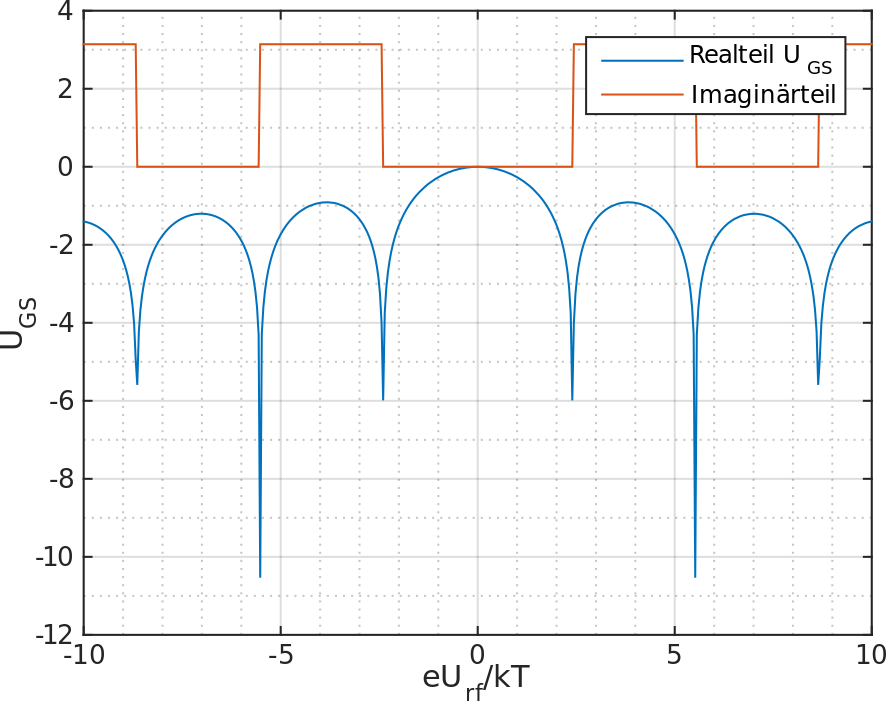
\includegraphics[width=\textwidth,height=0.8\textwidth]{figs/selfbiasselbst.png}
									\caption{}
									\label{img:imagundreal}
								\end{subfigure}
								\begin{subfigure}[t]{0.45\textwidth}
									\centering
									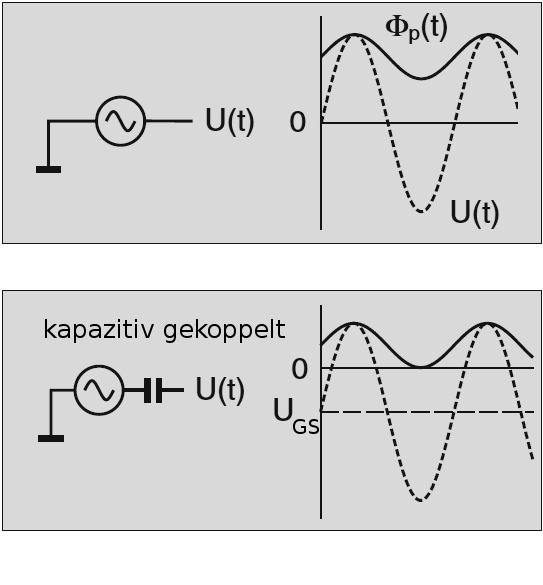
\includegraphics[width=0.7\textwidth,height=0.7\textwidth]{figs/kapazitivekopplungohneschemapiel.png}
									\vspace{-0.1cm}
									\caption{}
									\label{img:kapazitivgekoppelt}
								\end{subfigure}
								\caption{\fett{(a)}:Gleichspannungsanteil \tilt{self-bias} bei gegebenen Spannungen der Anregung $U\ix{rf}$, siehe Gl. (\ref{eq:selfbiasdrei}). \mbox{\fett{(b)}: Schema des} Potential- und Spannungsverlauf einer direkt und kapazitiv gekoppelten \tilt{rf}-Elektrode (nach \cite{Piel10}).}
						\end{figure}

		\subsection{Grenzschichten einer Entladung}\label{sub:rand}

			Im Hauptvolumen eines Plasmas werden die Neutralgasatome durch Wechselwirkungen mit den Elektronen zur Fluoreszenz angeregt. Die Grenzschichten von Gasentladung zu Metallen sind jedoch dunkler, als das eigentliche Plasma. Dies ist somit auf einen Elektronenmangel zur\"uckruf\"uhren, ähnlich wie in Abschn. \ref{subsub:verschieb} argumentiert. Die Quasineutralit\"at kann dort somit nicht mehr gelten. Es folgt, dass eine Randschicht automatisch eine positive Raumladungszone ist. \\
			Auf Grund der wesentlich gr\"o{\ss}eren Beweglichtkeit $\mu\ix{e}$ und thermischen Geschwindigkeit $v\ix{th,e}$, wird eine Wand in einem Plasma h\"aufiger von Elektronen getroffen, als von den korrespondierenden Ionen. Betrachtet man nur die Oberfl\"ache dieser, so kann man dessen Aufladung und damit auch das Potential $\Phi$ als negativ annehmen.

		\subsubsection{Child-Langmuir-Gesetz} \label{subsub:childlang}

		Die negative Aufladung einer Wand in einem Plasmas soll nun eine große Potentialbarriere gegen thermische Elektronen erzeugen, e.g. $|\Phi\left(0\right)-\Phi\left(-d\right)|\ll k\ix{B}T\ix{e}/e\,$. Die Betrachtung in einer Dimension soll hier genügen - es lässt sich leicht der dreidimensionale Zusammenhang daraus erweitern. Die Elektronendichte $n\ix{e}\left(x\right)$ geht mit dem Boltzmann-Faktor $f\ix{B}\left(\Phi\right)$ ("`\tilt{boltzmann-artige}"' Elektronen) wie

			\begin{align}
				n\ix{e}\left(x\right)=n\ix{e}\left(-d\right)f\ix{B}\left(\Phi\right)=n\ix{e}\left(-d\right)\exp\left(\frac{e\left(\Phi\left(x\right)-\Phi\left(-d\right)\right)}{k\ix{B}T\ix{e}}\right) \, .
			\end{align}

		Die Elektronendichte fällt damit exponentiell in Richtung der Wand ab. Das bedeutet, dass nur noch vorrangig Ionen ungehindert einströmen können. Es ist anzunehmen, dass die Randschichtausdehnung $d\ll\lambda\ix{mfp}$ die mittlere freie Weglänge des Plasma ist und die Ionen stoßfrei darin eintreten.\\
		An der Grenze zur Vorschicht (siehe \ref{img:dichterand}) haben die Ionen die Geschwindigkeit $v\ix{I,0}$ und das Potential der Wand verschwindet gerade an dieser Stelle. Für den Dichteverlauf der Ionen folgt:

			\begin{align}
				n\ix{I}\left(x\right)=n\ix{I}\left(-d\right)\left(1-\frac{2e\Phi\left(x\right)}{m\ix{I}v\ix{I,0}^2}\right)^{\frac{1}{2}}
			\end{align}

		Nimmt man weiterhin an, dass die kinetische Energie $m\ix{I}v\ix{I,0}^2/2\ll |e\Phi\left(x\right)|$ die Beschleunigung in der Randschicht ist, folgt somit die Bestimmungsgleichung (\ref{eq:potential}) für $\Phi\left(x\right)$ nach Poisson. Um dabei das korrekte Potential in der Grenzschicht zu erhalten, muss die Rückwirkung der Ionen auf dieses beachtet werden.

			\begin{align}
				\Delta\Phi\cong-\frac{en\ix{I}\left(-d\right)}{\varepsilon\ix{0}}\left(-\frac{2e\Phi\left(x\right)}{m\ix{I}v\ix{I,0}^2}\right)^{-\frac{1}{2}} \label{eq:potential}
			\end{align}

		Die klassische Lösung nach \tilt{Langmuir} für das eindimensionale $\Phi\left(x\right)$ erhält man aus Gl. (\ref{eq:potential}), wobei der ungestörte Ionenstrom geschrieben wurde als $j\ix{I}=n\ix{I}\left(-d\right)ev\ix{I,0}$.

			\begin{align}
				\Phi\left(x\right)=\left(\left(\frac{3}{4}\left(x+d\right)\right)^4\left(\frac{j\ix{I}}{\varepsilon\ix{0}}\right)^2\frac{m\ix{I}}{2e}\right)^{\frac{1}{3}}  \label{eq:langmuirpot}
			\end{align}

		Die Auflösung von Gl. (\ref{eq:langmuirpot}) nach dem Ionenstrom $j\ix{I}$ ergibt das \tilt{Child-Langmuir-Gesetz} ( Gl. (\ref{eq:childlang})). Dieses gibt nunmehr an, wie der Ionenstrom in der Randschicht von den Eigenschaften des ungestörten Plasmas abhängt. Umgekehrt bedeutet das, dass die Grenzregion auf Variationen des Potentials und der Parameter mit Veränderungen der Schichtdicke reagiert und damit versucht, den Einschränkungen der positiven Raumladungszone und dessen Ionenstrom nach dem \tilt{Child-Langmuir-Gesetz} zu genügen.

			\begin{align}
				j\ix{I}=\frac{4}{9}\varepsilon\ix{0}\left(\frac{2e\left(\Phi\left(-d\right)-\Phi\left(0\right)\right)^3}{m\ix{I}d^2}\right)^{\frac{1}{2}} \label{eq:childlang}
			\end{align}

				\begin{figure}
					\centering
					\begin{subfigure}[b]{0.6\textwidth}
						\centering
						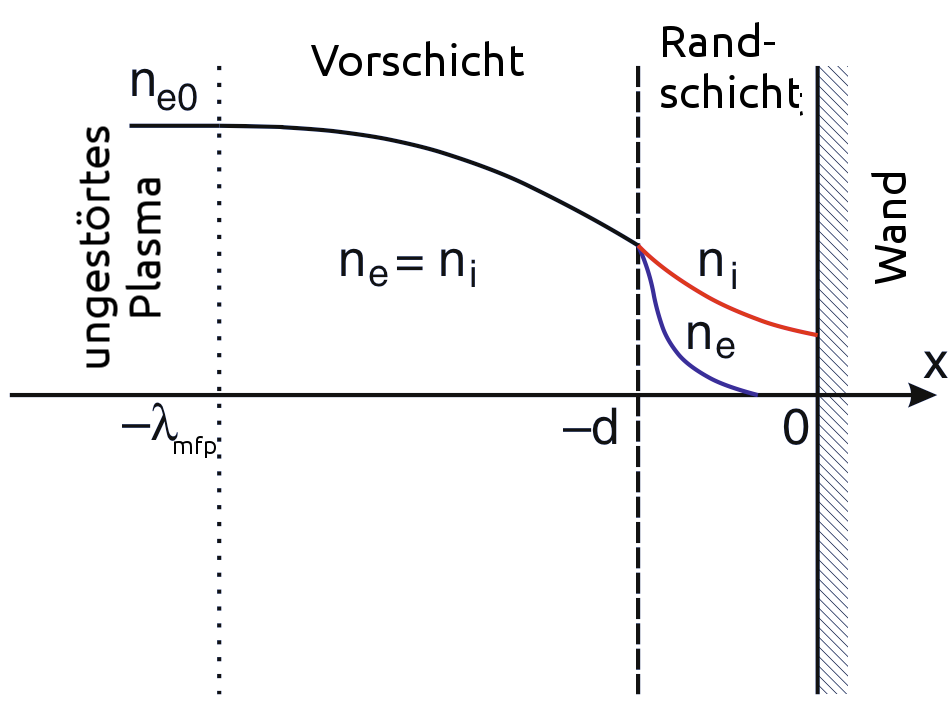
\includegraphics[width=0.7\textwidth,height=0.5\textwidth]{figs/randschichtpiel.png}
						\caption{}
						\label{img:dichterand}
					\end{subfigure}
					\begin{subfigure}[b]{0.375\textwidth}
						\centering
						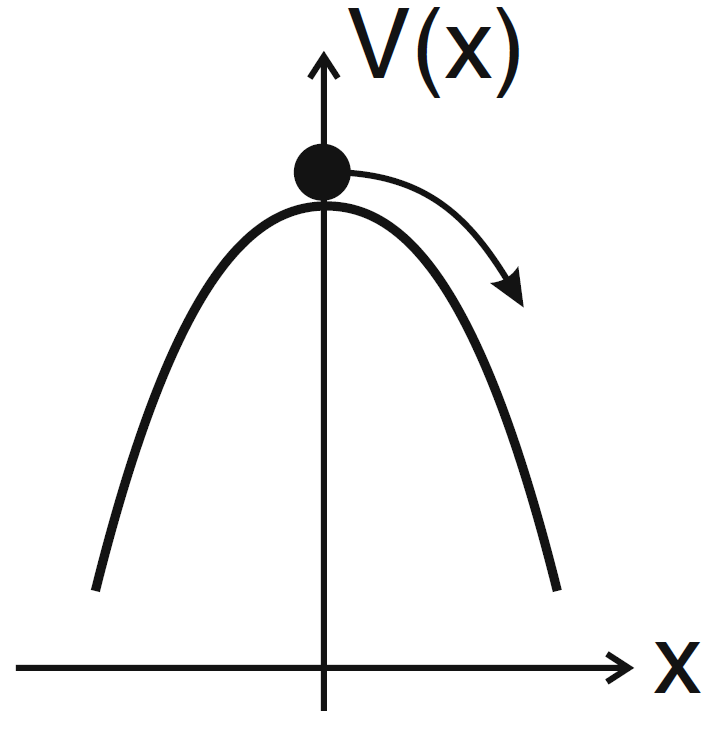
\includegraphics[width=0.8\textwidth,height=0.8\textwidth]{figs/parabelpiel.png}
						\caption{}
						\label{img:parab}
					\end{subfigure}
					\caption{\fett{(a)}: Dichten-Verlauf in der Grenzschicht zu einer Metalloberfläche. In einer bestimmten Entfernung $d$ zur Wand fällt die Elektronendichte praktisch auf 0, woraus die lokale Aufhebung der Quasineutralität folgt. \fett{(b)}: (Eindimensionales) Harmonisches Potential mit extremaler Instabilität. Kleine Auslenkungen sorgen für große Kräfte (nach \cite{Piel10}).}
				\end{figure}

		\subsubsection{Bohm-Kriterien}

			In Abschnitt (\ref{subsub:childlang}) wurde das Verhalten der Dichten der Ladungstr\"ager in einer Grenzschicht diskutiert. Diese erf\"ullen, in einem Abstand $d$ zur Wand in einem Plasma, die Eigenschaft der Quasineutralit\"at, welche weiterhin im Hauptvolumens gilt, nicht mehr. Es damit kein Kriterium f\"ur die Elektronen, welches sie daran hindert, auch aus weiten Teilen des Plasmas auf die Wand einzustr\"omen. Man stellt sich somit die Frage: Warum dehnt sich die Randschicht nicht in die gesamte Entladung aus? Wieso ist der Bereich der Elektronenersch\"opfung f\"ur eine Kombination der Plasmaparameter konstant? \\
			Um dieses Problem zu L\"osen, stellt man sich ein (mechanisches) Ein-Teilchen-Problem vor, bei welchem eine Gleichgewichtsanalyse vorgenommen wird. Das Potential habe ein Extremum - maximal oder minimal - an welchem die Punktmasse sich befindet. F\"ur den vorliegenden Fall des Randschicht-Problems sind nur Potentiale mit umgekehrt-parabelartigen Maxima interessant (siehe \ref{img:parab}), womit aus einer kleinen St\"orung eine gro{\ss}e Kraft auf das Teilchen folgt. In diesem Fall kann man also von einer Instabilit\"at sprechen.\\
			Der Bezug zur Plasmarandschicht wird deutlich, wenn man die Differentialgleichung des mechanischen Problems mit der Poissongleichung des Potentials in der Rand- bzw. Vorschicht - siehe Gl. (\ref{eq:pseudo}) vergleicht. Dabei stellt $\Psi\left(\Phi\right)$ ein Pseudopotential dar, welches in seiner Bedeutung vergleichbar mit der mechanischen Variante $V\left(\vec{r}\right)$ ist.

				\begin{align}
					m\frac{\diff^{2}\vec{r}}{\diff t^{2}}=-\frac{\diff V}{\diff\vec{r}} \quad \Leftrightarrow \quad \Delta_{\vec{r}}\,\Phi=-\frac{\diff\Psi}{\diff\Phi}=f\left(\Phi\right)\hspace{-0.3cm}\overset{Poisson}{\overset{\mid}{=}}\hspace{-0.3cm}\frac{\rho}{\varepsilon\ix{0}} \label{eq:pseudo}
				\end{align}

			Damit eine Instabilit\"at vorliegen kann, muss die, aus einer St\"orung des Pseudopotentials resultierende Kraft mit der Entfernung zum Gleichgewicht anwachsen. Die mathematisch \"aquivalente Formulierung ist die Ungleichung  in (\ref{eq:beding}). Nach Gl. (\ref{eq:pseudo}) und der in Abschnitt (\ref{subsub:childlang}) hergeleiteten Dichten in der Grenzschicht, kann die geforderte Bedingung \"uberpr\"uft werden. Aus ihr folgt das erste \tilt{Bohm-Kriterium}.

				\begin{align}
					0>\left.\frac{\diff^{2}\Psi}{\diff\Phi^{2}}\right|_{\Phi=0}\overset{Gl. (\ref{eq:pseudo})}{\overset{\mid}{=}}\left.\frac{\diff}{\diff\Phi}\left(\frac{n\ix{e}\left(x\right)-n\ix{I}\left(x\right)}{\varepsilon\ix{0}}\right)\right|_{\Phi=0}&=\frac{en\ix{e}\left(-d\right)}{\varepsilon\ix{0}}\left(\frac{e}{k\ix{b}T\ix{e}}-\frac{e}{m\ix{I}v\ix{0,I}^{2}}\right) \label{eq:beding} \\
					\Rightarrow \quad v\ix{0,I}\ge v\ix{B,I}=\sqrt{\frac{k\ix{B}T\ix{e}}{m\ix{I}}}& \label{eq:bohmkriteins}
				\end{align}

			($v\ix{B,I}$ - \tilt{Bohm}-Geschwindigkeit; $v\ix{0,I}$ - Ionen-Driftgeschwindigkeit; $T\ix{e}$ - Elektronentemperatur; $m\ix{I}$ - Ionenmasse)\\
			Für das Bohm-Kriterium in Gl. (\ref{eq:bohmkriteins}) kann auch analog die sog. \tilt{Machzahl} $M=v\ix{0,I}/v\ix{B,I}$ angegeben werden.\\
			Um zu erläutern, warum die Randschicht sich als Rückwirkung nicht in das Plasma ausdehnt, betrachten wir die Teilchenbewegung aus der Vor-Randschicht. Hier existiert ein elektrisches Feld, welches die Ionen auf die Geschwindigkeit $v\ix{B}$ in Richtung Wand beschleunigt. Außerdem gilt in ihr noch die Quasineutralitäts-Bedingung:

				\begin{align}
					n\ix{I}\left(x\right)=n\ix{I,0}\exp\left(\frac{e\Phi\left(x\right)}{k\ix{B}T\ix{e}}\right)=n\ix{e}\left(x\right)\,\, .
				\end{align}

			Hierbei ist $\Phi\left(x\right)$ das Potential der Vorschicht aus Abschnitt  (\ref{subsub:childlang}). 
			Da Stöße der Frequenz $\nu\ix{N,I}$ der Ionen mit den Neutralgasatomen einen nicht vernachlässigbaren Einfluss auf deren Strom haben, muss die Geschwindigkeitsverteilung umgeschrieben werden.

				\begin{align}
					\frac{\diff v\ix{I}}{\diff x}=\frac{\nu\ix{N,I}v\ix{I}^2}{v\ix{B}^2-v\ix{I}^2} \label{eq:geschwindverteil}
				\end{align}

			Aus der Singularität von Gl. (\ref{eq:geschwindverteil}) in $v\ix{I}=v\ix{B}$ und der Kenntnis über das Wandpotential lässt sich die Ausdehnung der Randschicht $d$ bestimmen. Offensichtlich werden Ionen mit einer Geschwindigkeit $v\ix{I}<v\ix{B}$ in der Vorschicht beschleunigt. Geschwindigkeiten größer als die Bohm-Geschwindigkeit kommen dort nicht vor, da dies nach Gl (\ref{eq:bohmkriteins}) nur in der Randschicht der Fall sein darf. \\
			Zusammen mit dem ersten \tilt{Bohm-Kriterium} folgt, dass am Übergang der Vor- zur Randschicht die Ionen $v\ix{B}$ erreichen müssen, damit sich eine positive Raumladungszone ausbilden kann.

				\begin{align}
					M=1 \quad \Leftrightarrow \quad v\ix{I}\left(-d\right)=v\ix{B} \label{eq:bohmkritzwei}
				\end{align}

			Lokal heißt das, dass bei $x=-d$ die Dichten bereits auf $\approx0,66n\ix{e,0}$ abgefallen sind (siehe \ref{img:dichterand}) und das Potential durch die Aufladung der Wand circa $-k\ix{B}T\ix{e}/2e$ beträgt.\\
			Ein Plasma "`sieht"' damit seine Randschicht nicht, da sich die notwendige Dynamik der entsprechenden Ladungsträger auf diese beschränkt und sich nicht beliebig ausdehnen kann. Mit anderen Worten: eine Randschicht bildet sich nur an Orten des Elektronenmangels und lokal negativer Potentiale aus.

		\subsection{Aufladung von Staubpartikeln}\label{sub:ströme}

			Die Ladung eines Fremdteilchens (Staub) in einem Plasma ist eine dynamische Größe. Sie ist zeitlich veränderlich, als auch abhängig von den Plasmaparametern, den Partikeleigenschaften sowie dessen Trajektorie in der Entladung. Offensichtlich ergibt sich die Ladung eines Teilchens zum Zeitpunkt $t$ aus den Ladungsströmen $I\ix{k}$ der Plasmaspezies auf das Partikel bis zu diesem Zeitpunkt. Im folgenden genügt es, dieses Problem auf einer Zeitskala zu betrachten, in der man die Ladung als konstant unter dem Einfluss der Ströme annehmen kann. Damit werden diese ebenfalls stationär und es gilt für ein einzelnes Teilchens die \tilt{Kirchhoff'sche Knotenregel}, wobei der Staub ein Knoten sei:

				\begin{align}
					\sum_{\text{k}} I\ix{k}\left(\Phi\ix{fl}\right)=\frac{\diff Q\ix{S}}{\diff t} \,\, . \label{eq:float}
				\end{align}

		Die Elektronen und Ionen im Plasma strömen aufgrund ihrer thermischen Bewegung auf das Fremdteilchen und verleihen diesem über Stöße eine Ladung $Q\ix{S}$, wobei sich für das Partikel ein elektrostatisches Potential $\Phi\ix{fl}$ einstellt, bei dem Gl. (\ref{eq:float}) gilt. Die Ladungsspezies kommen dabei im allgemeinen aus Sekundär-,Photo-, oder Feldemissionen, wobei die dominanten Ströme die des Plasmas selbst sind. Hier soll es ausreichen, die Plasmaströme nach  \tilt{Langmuir} und \tilt{Mott-Smith} mit dem sog. \tilt{orbital motion limit}-Modell \cite{Langmuir26} zu beschreiben. 

			\subsubsection{OML-Modell}\label{subsub:oml}

						\begin{figure}
							\centering
							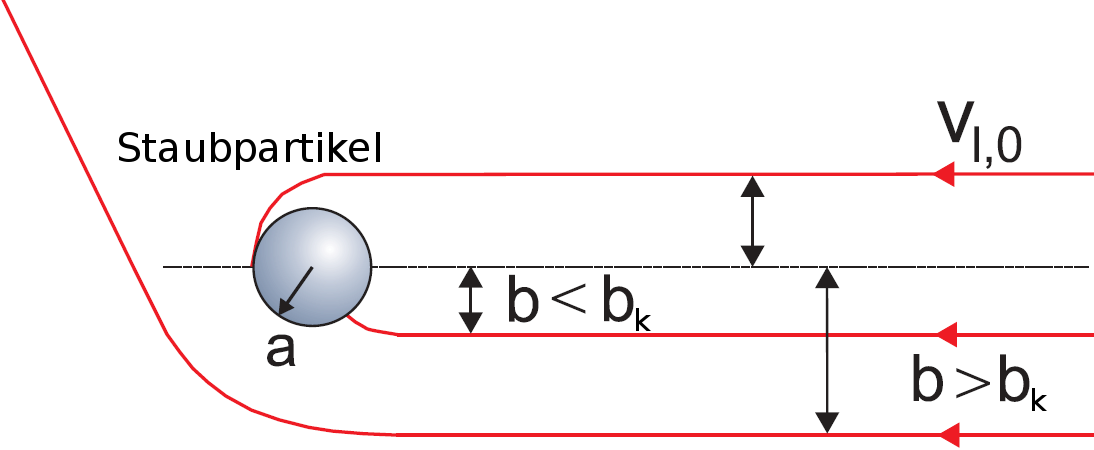
\includegraphics[width=0.7\textwidth, height=0.3\textwidth]{figs/orbitalmotionlimitmelzer.png}
							\caption{OML-Beschreibung eines, auf ein Staubpartikel einströmendes Ions. Der kritische Stoßparameter, für welcher eine Kollision stattfindet, ist $b\ix{k}$. Er ist im Vergleich zum geometrischen Querschnitt aufgrund der Coulomb-Wechselwirkung vergrößert (nach \cite{Melzer12}).}
							\label{img:oml}
						\end{figure}

			Dabei wird angenommen, dass sich ein strömendes Teilchen, welches zu $Q\ix{S}$ beiträgt bzw. damit elektrostatisch wechselwirkt, stoßlos aus dem Unendlichen (durch die Entladung) darauf zu bewegen kann. Aufgrund der, im allgemeinen höheren Elektronentemperatur und -beweglichkeit wird $\Phi\ix{fl}<0$, woraus eine veränderte Wechselwirkung mit den Teilchen der Ladungsströme folgt. Man definiert folglich einen kritischen Stoßparameter $b\ix{k}$, welcher dem Abstand eines Ions zur Target-Achse entspricht, bei dem dieses durch die Coulomb-Anziehung des Partikels gerade noch dessen Oberfläche tangiert. Für Parameter $b>b\ix{k}$ wird ein eintreffendes Ion auf seiner Trajektorie nur abgelenkt, für $b<b\ix{k}$ landet dieses auf dem Staubteilchen.\\
			Da vorausgesetzt wurde, dass keine Stöße vor dem Target geschehen, kann die Impulserhaltung zusammen mit der Energieerhaltung für ein einzelnes Projektil aufgestellt werden, welches sich im Abstand $b\ix{k}$ darauf zu bewegt:

				\begin{align}
					|\vec{L}|=|\vec{r}\times\vec{p}|=m\ix{I}v\ix{I}a=m\ix{i}v\ix{i,0}b\ix{k} \label{eq:impulserhaltung} \\
					E\ix{I}=\frac{m\ix{I}}{2}v\ix{I}^2+e\Phi\ix{fl}=\frac{m\ix{I}}{2}v\ix{I,0}^2 \label{eq:energieerhaltung}
				\end{align}

			In Gl.(\ref{eq:impulserhaltung}) und (\ref{eq:energieerhaltung}) stehen jeweils die linken Seiten für den Zeitpunkt des Auftreffens und die rechten für das Einlaufen aus dem Unendlichen. Durch Umformungen lässt sich ein Ausdruck für den kritischen Stoßparameter, in Abhängigkeit vom Partikelradius und dem \tilt{floating}-Potential aufgestellt werden.

				\begin{align}
					b\ix{k}^2=a^2\left(1-\frac{e\Phi\ix{fl}}{\frac{m\ix{I}}{2}v\ix{I,0}^2}\right) \label{eq:krit}
				\end{align}

			Der zugehörige Streuquerschnitt für die Streuung eines Teilchenstroms an einem Staubpartikel wird damit zu $\sigma\ix{k}=\pi b\ix{k}^2$, welcher größer als die geometrische Querschnittsfläche $\pi a^2$. Dem liegt die Coulomb-Wechselwirkung der Stoßpartner zu Grunde.\\
			Der (differentielle) Ladungsträgerstrom $\diff I\ix{j}$, welcher schließlich den Parameter der Partikelladung bestimmt, ergibt sich aus der Aufsummierung aller Stromdichten von Teilchen der Geschwindigkeiten $v\ix{j}$, gewichtet mit ihren zugehörigen Wechselwirkungsquerschnitten $\sigma\ix{j}$ und (hier: maxwellartigen) Verteilungen $f\left(v\ix{j}\right)$:

				\begin{align}
					\diff I\ix{j}=\sigma\ix{j}&\left(v\ix{j}\right)n\ix{j}v\ix{j}f\left(v\ix{j}\right)\diff v\ix{j} \nonumber \\
					\text{Ionen: } I\ix{I}&=\pi a^2n\ix{I}e\sqrt{\frac{8k\ix{B}T\ix{I}}{\pi m\ix{I}}}\left(1-\frac{e\Phi\ix{P}}{k\ix{B}T\ix{I}}\right) \label{eq:ionenstrom} \\
					\text{Elektronen: } I\ix{e}&=-\pi a^2n\ix{e}e\sqrt{\frac{8k\ix{B}T\ix{e}}{\pi m\ix{e}}}\exp\left(\frac{e\Phi\ix{P}}{k\ix{B}T\ix{e}}\right) \label{eq:elektronenstrom}
				\end{align}

			($T\ix{e,I}$ - Elektronen-/Ionentemperatur; $n\ix{e,I}$ - Elektronen-/Ionendichte, $\Phi\ix{P}$ - Partikelpotential; $k\ix{B}$ - \tilt{Boltzmann}-Konstante )\\
			Der Unterschied zwischen Gl. (\ref{eq:ionenstrom}) und (\ref{eq:elektronenstrom}) resultiert aus den unterschiedlichen Arten der Wechselwirkung mit dem Staubteilchen. Da $\Phi\ix{P}<0$ ist, werden Ionen aller Geschwindigkeiten in Richtung des Partikels gelenkt und könnten theoretische damit stoßen (respektiv der Geschwindigkeitsverteilung und dem Streuquerschnitt). Die Elektronen hingegen müssen mindestens eine Geschwindigkeit $v\ix{min}=\sqrt{-2e\Phi\ix{P}/m\ix{e}}$ besitzen, damit sie die Potentialbarriere zum Partikel überwinden und damit stoßen können. Au{\ss}erdem finden sich mit $\sqrt{8k\ix{B}T\ix{j}/\pi m\ix{j}}$ die thermischen Geschwindikeiten der jeweiligen Spezies $j$ als Vorfaktoren wieder. Damit werden die Gesamtstr\"ome letztendlich zum Produkt aus ungest\"orter, thermischer Stromdichte und der angepassten Wechselwirkungsfl\"ache des Partikels. \\
			Es sei erwähnt, dass aufgrund der hohen Teilchendichten in einem Plasma die OML-Theorie nicht der Realität entspricht. Die mittlere freie Weglänge eines Ions oder Elektrons hat in etwa die Dimension der Debyelänge $\lambda\ix{D}$ und ist nicht, wie vorausgesetzt, unendlich groß. Des weiteren entsprechen die $f\left(v\ix{j}\right)$ in der Praxis nicht isotropen Maxwell-Geschwindigkeitsverteilungen.

			\subsubsection{Neutralgas-Ionen-Stöße}

			Auf Grundlage der OML-Theorie lässt sich ein erweiterter Ausdruck für den Ionenstrom mit Rücksicht auf Stöße des Neutralgases aufstellen. Offensichtlich geht, mit dem Durchgang eines Projektils durch das Neutralgas einer Entladung, der Verlust kinetischer Energie einher. Es ist nun leicht nachzuvollziehen, dass sich viele Ionen, aufgrund der Ablenkungen durch Stöße und Wechselwirkung, um das negativ geladene Staubpartikel sammeln.
			\\In einer Sphäre mit dem Radius $R$ um das Teilchen ist die Stoßwahrscheinlichkeit zwischen Ionen und Neutralgasatomen

				\begin{align}
					\frac{R}{l\lambda\ix{mfp}}=Rn\ix{N}\sigma\ix{I,N} \,\, . \label{eq:wahrschein}
				\end{align}

			($n\ix{N}$ - Neutralgasdichte; $\sigma\ix{I,N}$ - Stoßparameter für Ion-Neutralgas-Stöße; \mbox{$\lambda\ix{mfp}$ - mittlere freie Wegl\"ange})\\
			Durch eine Sph\"are mit diesem Radius flie{\ss}t nun neben dem thermischen Ionenstrom $I\ix{th}$ noch ein weiterer Strom $I\ix{S}$ auf Grund der St\"o{\ss}e mit dem Neutralgas. Die Ionen der Geschwindigkeit $v\ix{th,I}$, welche sich ohne Wechselwirkung mit dem Gas der Entladung am Target vorbei bewegen w\"urden, werden mit der Sto{\ss}wahrscheinlichkeit aus Gl. (\ref{eq:wahrschein}) in Richtung des Staubteilchens abgelenkt und tragen somit zum Ladungsstrom auf dieses bei. Der Gesamtladungsstrom durch Ionen entspricht der Summe der beiden Str\"ome:

				\begin{align}
					I\ix{th}=&\pi R^{2}n\ix{N}ev\ix{th,I} \quad I\ix{S}=\pi R^2n\ix{N}ev\ix{th,I}\left(Rn\ix{N}\sigma\ix{N,I}\right) \\
					&I\ix{ges}=\pi a^{2}n\ix{I}ev\ix{th,I}\left(1-\frac{e\Phi\ix{P}}{k\ix{B}T\ix{I}}+\frac{R^{3}}{\lambda\ix{mfp}a^{3}}\right)
				\end{align}

			Auf der Oberfl\"ache der '\tilt{Sto{\ss}sph\"are}' $\mathbb{S}\ix{R}$ hat das \tilt{Yukawa}-Potential des Staubteilchens gerade die Energie der thermischen Ionenbewegung (Gl. (\ref{eq:bestimmR})), womit diese gerade noch in dessen Einfang geraten. Mit dem daraus bestimmten $R$ folgt ein diskreter Ionenstrom auf das Partikel mit R\"ucksicht auf die Ionen-Neutralgaswechselwirkung (Gl. (\ref{eq:ionstromkorr})).

				\begin{align}
					\frac{k\ix{B}T\ix{I}}{e}=&\frac{Z\ix{S}e}{4\pi\varepsilon\ix{0}R}\exp\left(\frac{R}{\lambda\ix{D}}\right) \label{eq:bestimmR} \\
					I\ix{I}=\pi a^{2} n\ix{I}e v\ix{th,I}&\left(1-\frac{e\Phi\ix{P}}{k\ix{B}T\ix{I}}+0,1\left(\frac{e\Phi\ix{P}}{k\ix{B}T\ix{I}}\right)^{2}\frac{\lambda\ix{D}}{\lambda\ix{mfp}}\right) \label{eq:ionstromkorr}
				\end{align}

			Im Vergleich zum Ergebnis des OML-Modells aus Gl. (\ref{eq:ionenstrom}) ist dieser Ladungstrom in Abh\"angikeit des Partikelpotentials und Ionentemperatur vergr\"o{\ss}ert. Die Wechselwirkung mit dem Neutralgas sorgt also, \"uber die St\"o{\ss}e und Erzeugung einer \tilt{Ionenwolke} um ein Teilchen, f\"ur einen gr\"o{\ss}eren pos. Ladungsstrom, welcher respektive wiederum f\"ur eine Steigerung des Elektronenstromes auf Grund des ver\"anderten Partikelpotentials sorgt. Eine selbstkonsistente L\"osung der, an den Anfang gestellte Problematik in Gl. (\ref{eq:float}) um das \tilt{floating}-Potential gestaltet sich jedoch als \"uberaus schwierig, da schon der OML-Theorie mehrere falsche Annahmen vorausgingen und dessen Eigenr\"uckwirkungen nicht-trivial sind.

		\subsection{Staub-Dynamik}\label{sub:dynamik}

			In einem Plasma wirken viele, u.U. nicht-triviale Kräfte auf den eingefangenen Staub. Im Folgenden werden die wichtigsten Einflüsse und Kenngrößen der Dynamik komplexer Plasmen vorgestellt und beschrieben. Insbesondere ist dieser Abschnitt wichtig für das Verständnis über die Bildung und Stabilität sog. \tilt{Yukawa-Cluster}. Dabei handelt es sich um ein System aus wenigen Staubteilchen, welche sich in einem äußeren, harmonischen Potential -  analog zum Schalenmodell des Atoms - anordnen. Diese sollen des Weiteren genauer in Abschnitt \ref{sub:yukawaclust} beschrieben werden.

			\subsubsection{Gravitation und elektrische Feldstärke}\label{subsub:grav}

			Betrachtet man ein Experiment, welches am Erdboden in Nähe der Meereshöhe durchgeführt wird, so muss offensichtlich die vollständige Gravitationskraft berücksichtigt werden. Dies gilt bspw. nicht für Versuche unter Mikrogravitation während Parabelflügen oder auf der \tilt{International Space Station}.

				\begin{align}
					F\ix{g}=m\ix{S} g=\frac{4}{3}\pi a^3 \rho\ix{S} g
				\end{align}

			($m\ix{S}$ - Masse der Staubteilchen; $a$ - Partikelradius; $\rho\ix{S}$ - Massendichte des Staubes; $g$ - \mbox{Erdbeschleunigung})\\
			Natürlich wirkt auf die, durch das ionisierte Gas elektrisch geladenen Partikel eine elektrische Kraft $F\ix{E}$, welche aus dem äußeren Feld $E$ der Plasma-Elektroden folgt. Eine elektrische Wechselwirkung mit dem Plasma tritt aufgrund der Quasineutralität nicht auf: innerhalb einer \tilt{Debye-Kugel} sind die Veränderung zu schnell, als dass das träge Staubteilchen diesen folgen könnte. 

				\begin{align}
				F\ix{E}=Q\ix{S} E=4 \pi \varepsilon\ix{0} a \Phi\ix{fl} E
				\end{align}

			($Q\ix{S}$ - Staubladung; $\Phi\ix{fl}$ - \tilt{floating}-Potential)\\
			Diese beiden Kräfte heben sich gerade in der Randschicht einer sog. Radiofrequenz-Entladung (\tilt{rf discharge}) auf, da sie für eine oben liegende Kathode antiparallel stehen. Zu beachten ist hierbei der stark unterschiedliche Einfluss des Teilchenradius - $\propto a^3$ und $\propto a$.\\

			\subsubsection{Abschirmung und Polarisationskräfte}\label{subsub:abschirm}

			Die große negative Aufladung der Staubteilchen sorgt über die Coulomb-Wechselwirkung mit den auf das Partikel zuströmenden Ionen dafür, das sich eine Konzentration derer lokal stark ändert. Es entsteht eine Wolke aus langsamen Ionen die quasi in der näheren Umgebung um das Teilchen verbleiben, jedoch nicht mit diesem interagiert und es nach außen hin vor dem Einfall schnellerer pos. Ladungen abschirmen. Somit gibt es keine direkte Rückwirkung der Wolke auf das Partikel, sofern dessen sphärische Symmetrie gegeben ist. Gilt dies nicht, so entsteht ein Multipol- bzw. Dipolmoment $\vec{p}$, welches danach strebt, sich in Richtung des Feldes $\vec{E}$ auszurichten. Damit wirkt eine Kraft $F\ix{Dip}$ (für ein Dipolmoment) auf das Staubteilchen zurück, welche mit dem Gradienten der Richtungsdifferenz zwischen $\vec{p}$ und $\vec{E}$ geht.

				\begin{align}
					\centering
					\vec{F}\ix{Dip}&=\vec{\nabla}\left(\vec{p}\vec{E}\right)\\
					&{\overset{\vec{p}\,||\vec{E}}{=}}\grad{pE} \nonumber
				\end{align}

			Das besagte Dipolmoment entsteht u.a. durch die diversen, gerichteten Ladungsprozesse in dem Plasma. Ein Partikel, welches in der Randschicht eingefangen und von einer Ionenwolke umgeben wird, 'sieht' unterschiedliche \tilt{Debye}-Längen über und unter sich aufgrund der lokalen Feldrichtung und der stark vom Mittelwert abweichenden Ionen- und Elektronendichten. Somit ändert sich offensichtlich die Plasmadichte innerhalb des Volumens einer Kugel mit dem, nun ortsabhängigen Radius $\lambda\ix{D}\left(\vec{r}\right)$. Insgesamt folgt daraus eine neue Bestimmungsgleichung für das Potential und damit auch eine neue Kraft $F\ix{E}$.

				\begin{align}
					\Delta \Phi\left(\vec{r}\right)-\frac{\Phi\left(\vec{r}\right)}{\lambda\ix{D}^2\left(\vec{r}\right)}=\frac{Q\ix{s}}{\varepsilon\ix{0}}\delta\left(\vec{r}\right) \\
					F\ix{E}=\underbrace{Q\ix{S}E}_{\text{(I)}}-\underbrace{\frac{Q\ix{S}^2}{8\pi\varepsilon\ix{0}}\frac{\nabla\lambda\ix{D}\left(\vec{r}\right)}{\lambda\ix{D}^2}}_{\text{(II)}}
				\end{align}

			Hierbei stellt (I) die normale Komponente dar und (II) ist zusätzliche Kraft durch die Deformation der Ionenwolke in Richtung kleinerer \tilt{Debye}-Längen $\lambda\ix{D}\left(\vec{r}\right)$. Die Kraft $F\ix{E}$ kann also dadurch größer oder kleiner werden. Hinzu kommt, dass der veränderte Parameter $\lambda\ix{D}$ von der Driftgeschwindigkeit $u\ix{I}$ abhängt, welche die Ionenwolke maßgeblich beeinflusst. Ist jedoch $u\ix{I}<v\ix{th,I}$ so kann man annehmen, dass die Ionenwolke besteht und $\lambda\ix{D}\left(\vec{r}\right)\approx\lambda\ix{D,I}$ gilt.\\
			Sind die Ionen jedoch schneller, womit $u\ix{I}>>v\ix{th,I}$ wird, so können sie nicht mehr vom Feld des Partikels 'gefangen' werden und damit die Ionenwolke bilden. So gilt folglich $\lambda\ix{D}\left(\vec{r}\right)\approx\lambda\ix{D,e}$.\\
			Insgesamt ist der Einfluss der Polarisation vernachlässigbar klein, solange die Teilchen eine Größe von einigen hundert $\unit{\mu m}$ nicht übersteigen.

		\subsubsection{Ionen-Neutralgasreibung}\label{subsub:reibung}

			Aufgrund der hohen negativen Ladung des Staubteilchens und der daraus resultierenden elektrostatischen Wechselwirkung existiert ein, relativ auf das Partikel zufließender, Ionenstrom oder auch "`Ionenwind"'. Weiterhin bewegen sich mit ihrer thermischen Geschwindigkeit die Neutralgasatome durch das Plasma und stoßen mit anderen Teilchen. Die Zahl der Stöße $\diff N$ einer Spezies mit einem Target mit dem Streuparameter $\sigma$ im Zeitintervall $\diff t$ ist somit über deren relative Geschwindigkeit $v\ix{rel}$ zu diesem in $\diff N=n\sigma v\ix{rel}\diff t$ gegeben. Hierbei kennzeichnet $n$ die Stromdichte der strömenden Teilchen. Aus diesem Strom folgt ein gewisser Impulsübertrag $\Delta p$ auf das Target. Hieraus lässt sich eine Kraft $F\ix{drag}$ ziehen, die einer Reibung bzw. einer Impulsaufnahme entspricht.

				\begin{align}
					F\ix{drag}=\frac{\diff N \Delta p}{\diff t}=\Delta p n \sigma v\ix{rel}
				\end{align}

			Man spricht hierbei auch von \tilt{ambipolarer Diffusion}, da die Ionenströme und damit auch die Ionenreibung zu beiden Polen führen. Man kann diese aus 2 Teilen aufbauen: direkte Kollisionen mit den Ionen $F\ix{dir}$ und deren Coulomb-Streuung an den Feldern der neg. geladenen Staubpartikel. Im folgenden soll das sog. \tilt{Barnes-Modell} eingeführt werden, welches die besagte Ionenreibung beschreibt.

				\paragraph{Ionenreibung: \tilt{Barnes-Modell}}

				Für die Bestimmung von $F\ix{dir}$ wird angenommen, dass nur die Ionen, welche für eine Ladungsänderung der Partikel sorgen, auch diese direkt treffen. Im Rückblick auf die Bestimmung der Ionenströme in \ref{sub:ströme} wird die Kraft durch Kollisionen zu

					\begin{align}
						F\ix{dir}=\pi a^2m\ix{I}\tilde{v}n\ix{I}u\ix{I}\left(1-\frac{2e\Phi\ix{fl}}{m\ix{I}\tilde{v}^2}\right)\,\,.
					\end{align}

				($n\ix{I}$ - Ionenkonzentration; $u\ix{I}$ - Ionen-Driftgeschwindigkeit; $m\ix{I}$ - Ionenmasse)\\
				Das Produkt aus Masse und mittlerer Geschwindigkeit der Ionen $m\ix{I}\tilde{v}=m\ix{I}\sqrt{u\ix{I}^2+v\ix{th,I}^2}$ entspricht dem Impulsübertrag.\\
				Für die Coulomb-Streuung müssen alle diejenigen Ionen miteinbezogen werden, welche mit dem Feld des Staubes 'stoßen'. Hierfür wird der Streuquerschnitt $\tilde{\sigma}$ der Ionen-Elektronen-Wechselwirkung auf den aktuellen Fall angepasst.

					\begin{align}
						\tilde{\sigma}=4\pi b_{\frac{\pi}{2}}^2\ln\left(\Lambda\right)=&\,4\pi b_{\frac{\pi}{2}}^2\ln\left(\frac{\lambda\ix{D}}{b_{\frac{\pi}{2}}}\right) \\
						\text{wobei }\, b_{\frac{\pi}{2}}=&\,\frac{e^2}{4\pi\varepsilon\ix{0}m\ix{I}v^2} \nonumber
					\end{align}

				Der Stoßparameter $b_{\frac{\pi}{2}}$ beschreibt eine Ablenkung um $\unit[90]{\degree}$. Für die Ionenreibung müssen weitere Bedingungen mit eingebunden werden: die Coulomb-Streuung außerhalb der Ionenwolke ist irrelevant, die Staubpartikel haben eine endliche Ausdehnung und damit existiert ein minimaler Stoßparameter $b\ix{k}$. Damit wird das gesuchte $\sigma$ zu

					\begin{align}
						\sigma=\int_{b\ix{k}}^{\lambda\ix{D}}\tilde{\sigma}\diff\left(\frac{\lambda\ix{D}}{b_{\frac{\pi}{2}}}\right)=&\,4\pi b_{\frac{\pi}{2}}^2\ln\left(\frac{\lambda\ix{D}^2+b_{\frac{\pi}{2}}^2}{b\ix{k}^2+b_{\frac{\pi}{2}}^2}\right)^{1/2} \nonumber \\
						F\ix{Coul}\overset{(*)}{=}&\,\frac{2\pi a^2 e^2\Phi\ix{fl}^2}{m\ix{I}\tilde{v}^3}n\ix{I}u\ix{I}\ln\left(\frac{\lambda\ix{D}^2+b_{\frac{\pi}{2}}^2}{b\ix{k}^2+b_{\frac{\pi}{2}}^2}\right)^{1/2} \, \, .
					\end{align}

				Den $\ln\left(\dots\right)$ nennt man auch den \tilt{Coulomb-Logarithmus} $\ln\left(\Lambda\right)$.\\
				In (*) wurde für die vollständige Coulomb-Kraft durch Ionen $F\ix{Coul}$ auf ein Partikel benutzt, dass dieses mit Ladung $Z\ix{S}e=Q\ix{S}$ als Kugelkondensator mit $Q\ix{S}=4\pi\varepsilon\ix{0}a\Phi\ix{fl}$ ausgedrückt werden kann. Wichtig zu beachten ist jedoch, dass nur Ionen einen Beitrag leisten, die innerhalb eines Stoßparameters $\lambda\ix{D}\approx\lambda\ix{D,e}$ am \tilt{target} vorbei fliegen.\\
				Die gesamte Kraft durch Ionen auf die Staubteilchen ist somit die Summe der Kräfte aus direkten Stößen und Coulomb-Kollisionen $F\ix{ion}=F\ix{dir}+F\ix{Coul}$, welche zusammen dargestellt sind in \ref{img:ionkräfte}.

					\begin{figure}
						\centering
						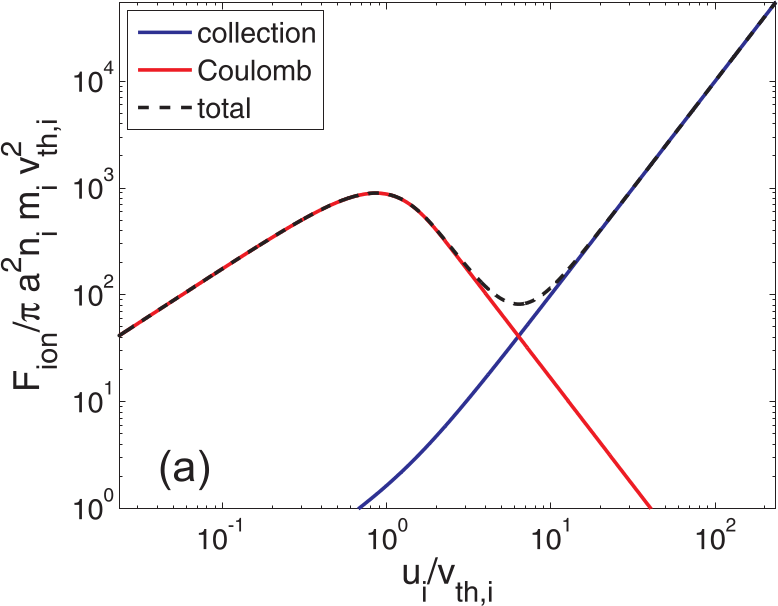
\includegraphics[height=0.4\textwidth,width=0.6\textwidth]{figs/forcesandtrappingmelzer.png}
						\caption{Berechnete Kräfte $F\ix{Coul}$ (\tilt{Coulomb}), $F\ix{dir}$ (\tilt{collection}) und die Summe beider auf einer doppelt-logarithmischen Skala(nach \cite{Melzer12}).}
						\label{img:ionkräfte}
					\end{figure}

		\subsubsection{Neutralgasreibung}

			Die Stöße mit den Neutralgasatomen können, ebenso wie die mit Ionen, als Kraft durch Reibung aufgefasst werden. Diese sorgen insbesondere für eine Verlangsamung der Bewegung der Staubteilchen. Die Kraft $F\ix{N}$ wird, in ähnlicher Weise wie $F\ix{dir}$, durch einen Impulsübertrag über einen Strom von Neutralgasteilchen auf einen effektiven Querschnitt ausgedrückt.

				\begin{align}
					F\ix{N}=-\delta\frac{4}{3}\pi a^3m\ix{N}v\ix{th,N}n\ix{N}v\ix{S}
				\end{align}

			($m\ix{N}$ - Neutralgasatommasse; $v\ix{th,N}$ - thermische Geschw. der Neutralgasatome; $n\ix{N}$ - Neutralgasdichte; $v\ix{S}$ - Staubteilchengeschw.)\\
			Der Faktor $\delta$ beschreibt hierbei die Art, wie die Neutralgasatome mit dem Staub stoßen. Eine spiegelnde Reflexion tritt für ein $\delta=1$ auf. Mit steigendem $\delta$ wird die Kollision immer diffuser, bis hin zu einem Wert von $\delta=1,44$.\\
			Für den berühmten \tilt{Milikan}-Öltropfen-Versuch zur Bestimmung der Ladung eines Elektrons wurde, 1924 von \tilt{P. S. Epstein}, ebenso ein Ausdruck für die Kraft durch Neutralgasreibung bestimmt. Dabei ist $\beta$ der Reibungskoeffiziént und $\rho\ix{S}$ die Dichte des Staubmediums.

				\begin{align}
					F\ix{N}=-m\ix{S}\beta v\ix{S}=-m\ix{S}v\ix{S}\delta\frac{8}{\pi}\frac{p}{a\rho\ix{S}v\ix{th,N}}
				\end{align}

		\subsubsection{Thermophoretische Kraft}\label{subsub:therm}

			In einer Plasmakammer kann, durch Aufheizung oder Abkühlung einer der Elektroden bzw. Kammerbegrenzungen ein, bspw. der Gravitation oder dem elektrischen Feld entgegen gerichteter Temperaturgradient angelegt werden.\\
			Die Kraft kann folgendermaßen erklärt werden: auf der Seite der höheren Temperatur haben die Neutralgasteilchen im Mittel eine größere Geschwindigkeit und Impuls, woraus ein positiver Impulsübertrag in Richtung niedrigerer Temperaturen folgt.	Mit der Wärmeleitfähigkeit des Neutralgases $\kappa\ix{N}$ folgt für die thermophoretische Kraft $F\ix{th}$ Gl. (\ref{eq:therm}). Auf Grund $\propto a^2$ ist diese Kraft besonders wichtig für Teilchen mit einem Radius kleiner als $\unit{\mu m}$. Sie wird für die Formation von sog. \tilt{Yukawa-Clustern} genutzt (siehe \ref{sub:yukawaclust}).

				\begin{align}
					F\ix{th}=-\frac{32}{15}\frac{a^2 \kappa\ix{N}}{v\ix{th,N}}\grad{T} \label{eq:therm}
				\end{align}

			Es sei erwähnt -  über die Zustandsgleichung für ideale Gase $pV=Nk\ix{B}T$ ersichtlich -, dass bei einer höheren Temperatur die Dichte des Neutralgases sinkt. Experimentell findet man daher, dass die verminderte Dichte zu einer niedrigeren Stoßintensität führt und damit den Effekt der Thermophorese in etwa gerade kompensiert. Trotzdem bleibt die Methode des Temperaturgradienten ein wichtiges Mittel zum Einfang des Staubes und Ausgleich der Gravitationskraft.

		\subsubsection{Kraft durch \tilt{Laser}-Einstrahlung}\label{subsub:laser}

			Der Einsatz von \tilt{Laser} (\fett{L}ight \fett{A}mplification by \fett{S}timulated \fett{E}mission of \fett{R}adiation) hat in Versuchen zu kolloidalen Plasmen verschiedene Gründe: einerseits wird der \tilt{target}-Bereich mit ihnen ausgeleuchtet, andererseits können unterschiedliche dynamische Eigenschaften des Staubes untersucht werden.\\
			Die Manipulation von eingefangenen Teilchen wird bspw. durch die Fokussierung eines \tilt{Laser}strahls auf ein Partikel realisiert. Hierbei spielt der Impulsübertrag der Photonen mit Impuls $p\ix{Ph}$, welcher dem Strahlungsdruck $p\ix{Strahl}$ entspricht und die photophoretische Kraft $F\ix{ph}$ eine Rolle.

				\begin{align}
					p\ix{Strahl}=\frac{\diff p\ix{ph}}{A\ix{L}\diff t}=&\frac{\diff N\ix{ph}}{A\ix{La}\diff t}\frac{h}{\lambda}=\frac{I\ix{L}}{c} \nonumber \\
					F\ix{Strahl}=&\gamma\frac{I\ix{L}}{c}\pi a^2 \label{eq:strahl}
				\end{align}

			($N\ix{ph}$ - Anzahl der, die das Partikel treffenden Photonen; $\lambda$,$\nu$ - Lasergrößen; $A\ix{L}$ - Querschnittsfläche des \tilt{Laser}; $\gamma$ - Wechselwirkungskoeffizient für den Stoß Photon-Staub)\\
			Für ein $\gamma=2$ in Gl. (\ref{eq:strahl}) liegt eine Totalreflexion vor, für $\gamma=1$ wird der Impuls der auftreffenden Photonen vollständig absorbiert. Ein \tilt{Laser}-Strahl kann u.a., auf Grund der anisotropen Photonendichte (\tilt{gaussian bandwidth}) über den Querschnitt, zum Einfang von (einem) ausgewählten Partikeln benutzt werden.
			Bei der photophoretischen Kraft wird die resultierende Dynamik aus dem, durch die Stöße mit Photonen erzeugten Temperaturgradienten über ein einzelnes Partikel beschrieben. Wie bereits erläutert, liegt ein Strahldichtegradient für eine Fläche von $A\ix{S}$ vor, woraus eine unterschiedliche Staubaufheizung durch die Stoßreibung folgt.\\
			Treffen nun Neutralgasatome auf die heißere Seite, so werden sie dort schneller reflektiert, als von der kälteren. Die Differenz des Impulsübertrags resultiert in der photophoretischen Kraft, die entgegen des Gradienten der Photonendichte und damit in Richtung der heißen Seite der Partikel zeigt. Je nach der Absorptionsfähigkeit besitzen die Teilchen unterschiedliche Temperaturgradienten. Somit stellt sich eine heiße Front aus den Teilchen auf, welche eine gute Absorption und somit insgesamt höhere Temperatur aufweisen. Für diese Partikel zeigt $F\ix{ph}$ in Richtung des Strahls. Analog wirkt die photophoretische Kraft für schlecht absorbierende Teilchen in entgegengesetzte Richtung. Somit ergibt sich $F\ix{ph}$ in Gl. (\ref{eq:photoph}) mit dem Wärmeleitungskoeffizienten $\kappa\ix{S}$ des Staubes, dem Gasdruck $p$ und der Gastemperatur $T$.

				\begin{align}
					F\ix{ph}=\frac{\pi a^2 p I\ix{L}}{6\left(pav\ix{th,N}+\kappa\ix{S}T\right)} \label{eq:photoph}
				\end{align}

		\subsubsection{Einfang und Gleichgewicht}\label{subub:einfang}

				\begin{figure}
					\centering
					\begin{subfigure}[t]{0.49\textwidth}
						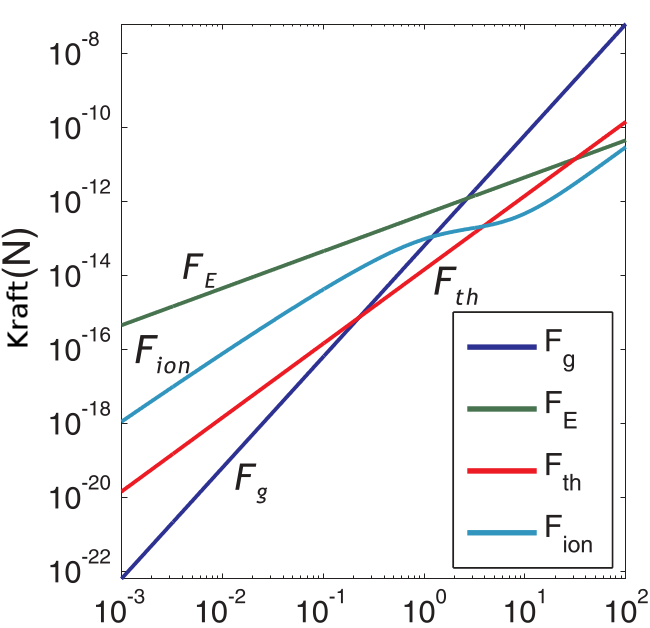
\includegraphics[width=\textwidth,height=\textwidth]{figs/allforcesequlibriummelzerlinks.png}
						\caption{}
						\label{img:linkseq}
					\end{subfigure}
					\begin{subfigure}[t]{0.49\textwidth}
						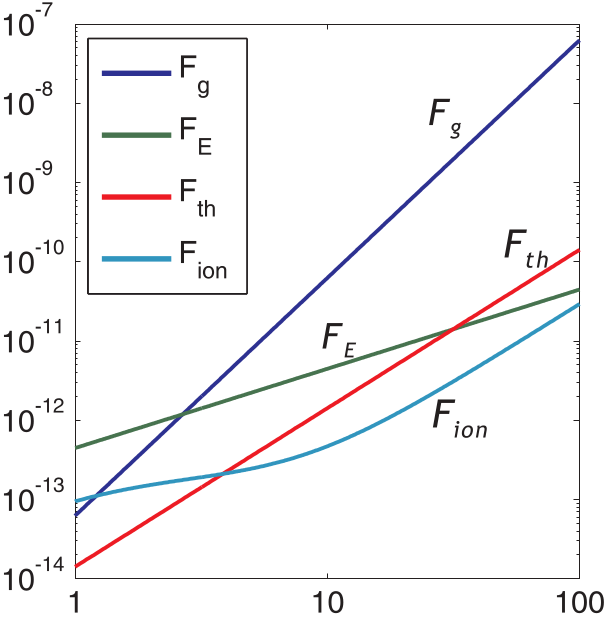
\includegraphics[width=\textwidth,height=\textwidth]{figs/allforcesequlibriummelzerrechts.png}
						\caption{}
						\label{img:rechtseq}
					\end{subfigure}
					\caption{Kräfte als Funktion des Teilchenradius in einem Argon-Plasma (Parameter: $\kappa\ix{N}=\unit[0,016]{\frac{kg m}{s^3}}$;  \mbox{$\rho\ix{S}=\unit[1,5\cdot\tenpo{3}]{\frac{kg}{m^3}}$}; $T\ix{e}=\unit[2]{eV}$; $\Phi\ix{fl}=\unit[-4]{V}$; $E=\unit[1000]{\frac{V}{m}}$; $n\ix{I}=\unit[\tenpo{5}]{m^{-3}}$; $u\ix{I}=v\ix{th,I}=v\ix{th,N}=\unit[400]{\frac{m}{s}}$, nach \cite{Melzer12}) }
					\label{img:kräfte}
				\end{figure}

			In \ref{img:kräfte} sind einige der bisher beschriebenen Kräfte für typische Parameter berechnet und mit einer doppelt-logarithmischen Skala dargestellt worden.\\
			Für Teilchen mit einem Radius im Bereich von einigen $\unit{\mu m}$ sind die Kräfte des äußeren elektrischen Feldes $F\ix{E}$ und der Gravitation $F\ix{G}$ dominant. Daher müssen, für einen praktikablen Einfang, diese beiden Kräfte im Gleichgewicht sein, d.h. sich stationär aufheben. Dies ist gerade in der nahen Randschicht der positiven Elektrode der Fall, da dort $F\ix{E}$ stark genug ist. Weil $\grad{E}\ll1$ ist, gilt dies nur lokal.\\
			Für $a\gg\unit[1]{\mu m}$ wird $F\ix{E}$ weniger relevant und es übt die Thermophorese eine immer größere Kraft auf den Staub aus. Genauer: $F\ix{th}$ ist in Experimenten sogar schon für $\grad{T}\approx \unit[2]{\frac{K}{m}}$ eine wichtige, nicht vernachlässigbare Größe. Für die Neutralgasreibung $F\ix{N}$ gilt, dass diese bei großen thermischen Geschwindigkeiten des Staubes nahezu konstant wird, jedoch für "`kalten"' Staub mit zunehmendem Drift $v\ix{S}$ an Einfluss gewinnt. Die Ionenreibung $F\ix{ion}$ ist unter diesen Umständen vergleichsweise klein.\\
			Sind die Staubpartikel klein, d.h. haben einen Radius $a\approx\unit[\tenpo{-9}]{m}$, so wird die Gravitationskraft mit ihrem Einfluss $\propto a^3$ sehr klein und spielt damit kaum noch eine Rolle. Damit muss die Kraft des elektrischen Feldes mit der Ionenreibung bzw. der Thermophorese balanciert werden.		

				\begin{figure}
					\centering
					\begin{subfigure}[b]{0.45\textwidth}
						\hspace{0.3cm}
						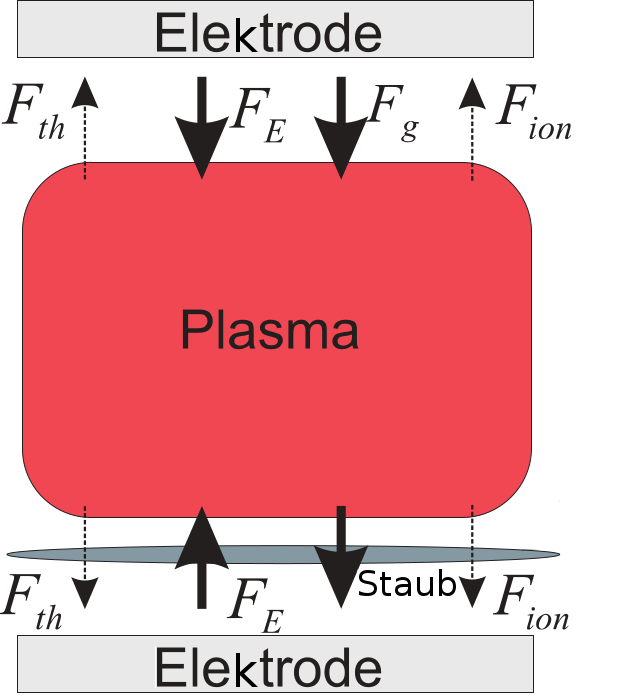
\includegraphics[width=\textwidth,height=\textwidth]{figs/directionsofforcesandtrappingmelzerlinks.png}
						\caption{}
						\label{img:linksdirection}
					\end{subfigure}
					\begin{subfigure}[b]{0.45\textwidth}
						\hspace{-0.2cm}
						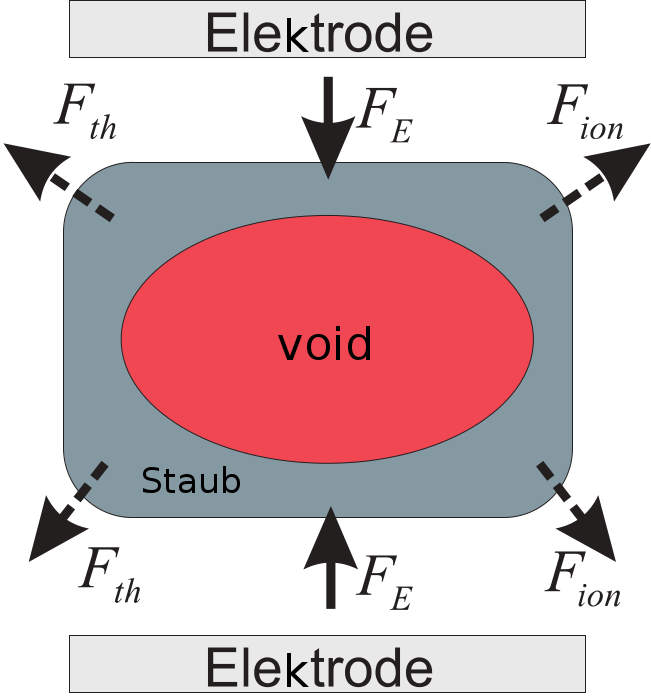
\includegraphics[width=\textwidth,height=\textwidth]{figs/directionsofforcesandtrappingmelzerrechts.png}
						\caption{}
						\label{img:rechtsdirection}
					\end{subfigure}
					\caption{Schemata für dein Einfang von Staub mit \fett{(a)}: $a\approx\unit[\tenpo{-5}]{m}$ (\fett{b)}: $a\approx\unit[\tenpo{-9}]{m}$ bzw. unter Mikrogravitation. Es wurden die wichtigsten Kräfte und deren Richtungen eingezeichnet (nach \cite{Melzer12}).}
					\label{img:kräfterichtungen}
				\end{figure}

			In \ref{img:kräfterichtungen} sind schematisch die Kräfte aus \ref{img:kräfte} mit ihren Orientierungen dargestellt worden. \\
			Abbildungsteil (a) zeigt dabei den Einfang von $\unit{\mu m}$-großen Teilchen in einer kleinen, lokalisierten Randschicht. Diese ordnen sich dabei in ausgedehnten Schichten mit hexagonaler Struktur (\tilt{fcc} bzw. \tilt{bcc}) an. Die Kräfte der Thermophorese und des "`Ionenwindes"' ($F\ix{ion}$) zeigen dabei aus dem Plasma heraus in Richtung der Kammer bzw. der Elektroden. Die Ionen sind dabei bestrebt, aufgrund der ambipolaren Diffusion in der Randschicht auf die Kammerwand, den Ladungsunterschied (etwa innerhalb einer \tilt{Debye}-Länge) zwischen dem Plasma und dem Gehäuse auszugleichen. Das liegt u.a. an den unterschiedlichen Beweglichkeiten der Ladungsträger und deren Strömung auf die Kammer (siehe Abschn. \ref{sub:rand}). Weiterhin gilt ähnliches für die thermophoretische Kraft: das aufgeheizte Plasma erzeugt einen Impulsübertrag in Richtung der kühleren Kammer, woraus eine Kraft vom Plasma weg folgt. Der Staub wird somit in einem Teil der Entladung eingefangen, in dem diese Kräfte eine untergeordnete Rolle spielen. Die relevante elektrische Feldkraft ist besonders in der Nähe der Elektroden groß und kann damit dort Gravitationskraft bzw. $F\ix{th}$ und $F\ix{ion}$ kompensieren. Sie zeigt zudem in Richtung des Plasmas, da dieses in der Randschicht nicht mehr als neutral betrachtet werden kann.\\
			Im zweiten Teil (b) von \ref{img:kräfterichtungen} ist ein Plasma mit Staubteilchen im $\unit{nm}$-Bereich unter Schwerelosigkeit gezeigt. Dabei entsteht der sog. \tilt{void}, welcher ein Fremdteilchen-freier Bereich in Mitten der Entladung ist und aufgrund der relativen Orientierungen der Kräfte zustande kommt. Thermophorese und Ionenwind-Kraft zeigen (selbe Argumentation wie zu Teil \fett{(a)}) aus der 'Mitte' des Plasma in Richtung der Kammer und der Elektroden, wobei von diesen aus die elektrische Feldkraft zum \tilt{void} zeigt. Da in diesem Fall $F\ix{G}$ sehr klein ist (wegen $\propto a^3$), muss für den Einfang des Staubes das starke $F\ix{E}$, welches zwischen Kammer und Plasma entsteht, mit $F\ix{th}$ und $F\ix{ion}$ im Gleichgewicht sein. Somit ist es m\"oglich, Staub in dreidimensional ausgedehnten Bereichen in der gesamten Entladung einzufangen.\\ Es stellen sich sogar Dichte- bzw. Volumen- und Massegradienten aufgrund der empfindlichen Abhängigkeit von Gravitation und elektrischer Feldkraft ein. Das bedeutet, dass sich schwerere, größere Teilchen bzw. "`verschmolzene"' Partikelcluster am Rande des Einfangs wiederfinden, wohingegen kleinerer Staub sich dicht gepackt um den \tilt{void} herum befindet.

		\subsection{Finite Yukawa-Cluster}\label{sub:yukawaclust}

				\begin{figure}[t]
					\centering
					\begin{subfigure}[b]{0.3\textwidth}
						\centering
						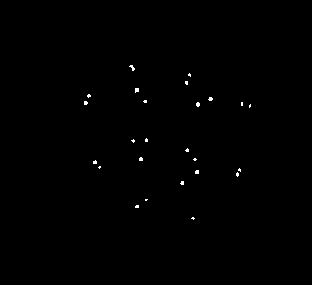
\includegraphics[width=\textwidth,height=\textwidth]{figs/rot00013ungestrt.png}
						\caption{}
						\label{img:rechts}
					\end{subfigure}
					\begin{subfigure}[b]{0.3\textwidth}
						\centering
						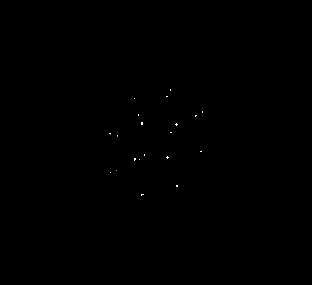
\includegraphics[width=\textwidth,height=\textwidth]{figs/gruen05006ungestrt.png}
						\caption{}
						\label{img:links}
					\end{subfigure}
					\begin{subfigure}[b]{0.3\textwidth}
						\centering
						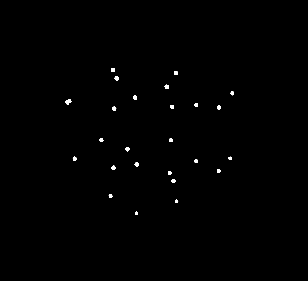
\includegraphics[width=\textwidth,height=\textwidth]{figs/gelb00011ungestrt.png}
						\caption{}
						\label{img:oben}
					\end{subfigure}
					\caption{Aufnahmen aus 3 verschiedenen, orthogonalen Raumrichtungen eines \tilt{Yukawa-Balls} mit $N=26$ Teilchen. Das System befindet sich bei niedrigen Gasdrücken ($\approx\unit[6-10]{Pa}$) in einer Argon-Entladung unter einem Kupferring, welcher sich im Plasma auf $\Phi\ix{fl}$ aufgeladen hat. \fett{(a)}: Ansicht aus der Ebene des Clusters \fett{(b)}: von oben \fett{(c)}: andere Richtung in der Ebene}
				\end{figure}

			Bisher wurden in den Abschnitten \ref{sub:kaprfplasm} und \ref{sub:rand} allgemein gültige Charakteristika des für diesen Aufbau verwendeten Plasmas besprochen. Außerdem sind in \ref{sub:ströme} und \ref{sub:dynamik} die für komplexe bzw. staubige Plasmen spezifischen Kenngrößen und Prozesse, wie beispielsweise Aufladung und Einfang, beschrieben worden. Damit kennen wir die Dynamik eines einzelnen Staubteilchen in einem Plasma und unter welchen Bedingungen ein Einfang gegeben ist, jedoch wissen wir nichts über das kollektive Verhalten der bereits besprochenen \tilt{Yukawa-Cluster}. Wann und wo sind diese - falls ein solcher Zustand existiert - stabil? Wie ist ihr Verhalten bei Störungen des externen Potentials? Dieser Abschnitt soll sich mit diesen Fragen, in Bezug auf einen Versuch unter den Bedingugen aus \ref{img:linksdirection}, auseinander setzen.

				 \subsubsection{Struktur}

						 \begin{figure}
						 	\centering
						 	\begin{subfigure}[t]{0.48\textwidth}
						 		\centering
						 		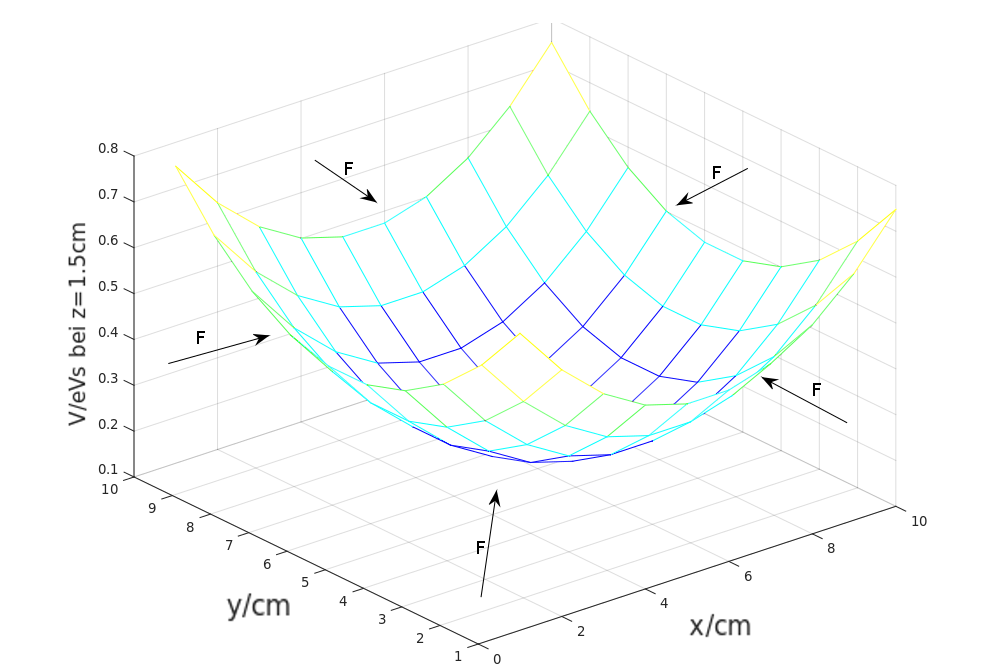
\includegraphics[width=1.1\textwidth,height=0.3\textheight]{figs/einfangpotnu.png}
						 		\caption{}
						 		\label{img:potential}
						 	\end{subfigure}
						 	\begin{subfigure}[t]{0.48\textwidth}
						 		\centering
						 		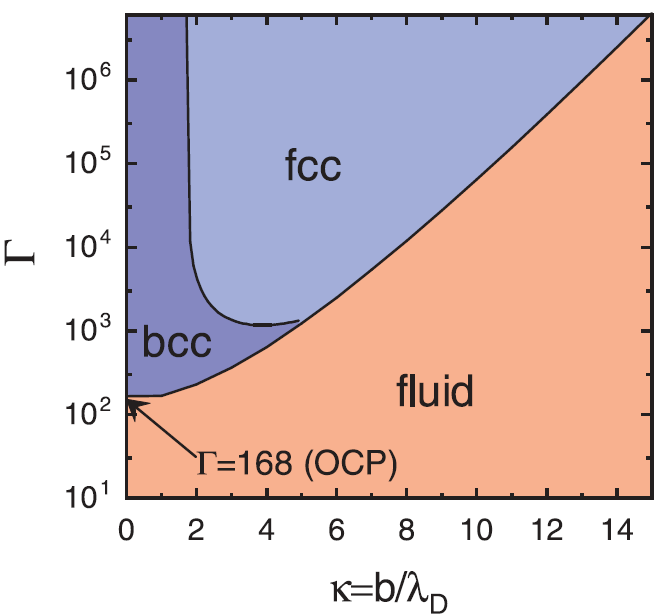
\includegraphics[width=0.9\textwidth,height=0.3\textheight]{figs/gammaphasetransmelzer.png}
						 		\caption{}
						 		\label{img:gamma}
						 	\end{subfigure}
						 	\caption{\fett{(a)}: Harmonischer Einfang des Potentials $V$ in $\unit{eVs}$ mit globalem Minimum (dunkel). Darstellung für eine Elektrodenhöhe (siehe später Abschnitt \ref{sub:einfang}) von $\unit[1,5]{cm}$. \fett{(b)}: Phasendiagramm nach \cite{Melzer12} für eine effektive Coulomb-Kopplung nach Gl. (\ref{eq:kopplung}).}
						 \end{figure}

					 Ein \tilt{Yukawa-Ball} kann durch das Erzeugen eines externen Potentials eingefangen werden: beispielsweise durch räumliche Begrenzung mit einer Küvette oder einem Ring, welche sich im Plasma aufladen und damit eine nach innen gerichtete, elektrische Kraft auf den ebenfalls negativ geladenen Cluster ausüben. Das aus den Kräften auf die Staubpartikel resultierende Potential kann als harmonisch angenommen werden, e.g.:

						 \begin{align}
						 	V\left(\vec{r}\ix{j}\right)=\frac{m\ix{S}\omega\ix{0}^2}{2}\begin{pmatrix} 1 \\ \alpha\ix{y}  \\ \alpha\ix{z} \end{pmatrix} \vec{r}\ix{j}^2
						 \end{align}

					,wobei $\alpha\ix{k}=\omega\ix{k}^2/\omega\ix{x}^2$ die relative der Richtung $k\in\left\lbrace x,y,z\right\rbrace$ und $\omega\ix{0}=\omega\ix{x}$ die absolute Einfangstärke ist. In \ref{img:potential} ist das Potential, in dessen globalen Minimums sich der Cluster in diesem Experiment bildet, für eine feste Höhe über der getriebenen Elektrode dargestellt. Für eine geeignete Anordnung strebt man einen isotropen Einfang mit $\omega\ix{x}=\omega\ix{y}=\omega\ix{z}$ an.\\
					Um ein Maß für die Stabilität eines staubigen Plasmas zu erhalten, geht man, wie bei Festkörpern und deren Elektronengasen, von einer Punktladung $Q$ vor dem Hintergrund der Ionen aus (\tilt{one component plasma} - OCP). Der Kopplungsparameter $\Gamma$ in Gl. (\ref{eq:kopplung}) beschreibt somit die elektrostatische Wechselwirkung eines Teilchens mit seinen Nachbarn in Einheiten der thermischen Energie. Für ein $\Gamma>1$ spricht man von einer starken Kopplung innerhalb des Clusters bzw. des Plasmas. Mit $\Gamma\geq\Gamma\ix{k}\simeq168$ liegen kristalline Systeme vor. Bei einem kleineren Wert gehen die Cluster in einen flüssigen bzw. gasförmigen Zustand über (\ref{img:gamma}). Das heißt, dass ein System aus Staubpartikeln "`schmelzen"' kann, bringt man durch Lasereinstrahlung o.ä. gezielt Energie in den Cluster ein und verringert damit die Ordnung bzw. erhöht die thermische Bewegung. Dabei verschwindet zuerst die Winkelabhängigkeit, was das Auflösen der kristallartigen Strukturen innerhalb des Clusters zur Folge hat (zum Beispiel \cite{Thomas96}).\\
					Die größe $b\ix{WS}=\left(3/4\pi n\ix{S}\right)^{-1/3}$ ist der \tilt{Wigner-Seitz}-Radius: er ist analog zu $\overline{b}$ aus Tab. \ref{tab:kenngroessen} eine Skala für Teilchenabstände. Insbesondere ist $b\ix{WS}$ eine korrektere Größe, da sich der Staub in hexagonalen bzw. pentagonalen Zellen auf den konzentrischen Sphären des Clusters anordnet. Die Zusammensetzung eines solchen, \tilt{finiten Yukawa-Systems} ähnelt stark dem Orbital- bzw. Schalenmodell der Atomphysik. Außerdem: sowohl aufgrund der bisher besprochenen Kräfte und der Coulomb-Wechselwirkung des Staubes, als auch wegen des nicht-reziproken \tilt{Ionenfokus} (siehe \cite{Melzer95c}) streben die Systeme eine energetisch günstige fcc- (\tilt{face centered cubic}) bzw. bcc-Struktur (\tilt{body centered cubic}) an.

						\begin{align}
							\Gamma=\frac{Z\ix{S}e^2}{4\pi\varepsilon\ix{0}b\ix{WS}k\ix{B}T\ix{S}}  \,\,; \quad \Gamma\ix{C,eff}=\Gamma\exp\left(-\frac{b\ix{WS}}{\lambda\ix{D}}\right) \label{eq:kopplung}
						\end{align}

					Der effektive Parameter reiner Coulomb-Wechselwirkungen $\Gamma\ix{C,eff}$ entspricht einer modifizierten Kopplung mit Rücksicht auf die Abschirmung durch die Ionenwolke (\cite{Lampe00}, \cite{Schweigert00d}) um ein Partikel bzw. den Cluster. Aus diesem Grund führt man die Abschirmstärke $\kappa=b\ix{WS}/\lambda\ix{D}$ ein, welche angibt, um wie viel die elektrostatische Wechselwirkung mit einem Teilchen der Ladung $Q$ innerhalb einer Elementarzelle der Staubpartikel abgeschwächt ist. Außerdem folgt daraus der Zusammenhang für die Phasengrenze in \ref{img:gamma} $\Gamma\left(\kappa\right)$: für große \tilt{Wigner-Seitz}-Radien bzw. sehr kleine Debye-Längen verschwindet die Wechselwirkung zwischen den Staubteilchen nahezu vollständig. Das Yukawa-Potential geht für diesen Fall in das harter Kugeln über (bspw. van-der-Waals-Gastheorie etc.).\\
					Abschließend sei erwähnt, das die bisher genannten Eigenschaften u.U. stark von der Art der Wechselwirkung bzw. der Teilchenzahl abhängen: die Betrachtungen vernachlässigen vollständig den Einfluss einer \tilt{Elektronenerschöpfung} (\cite{Melzer07}) und gehen von reiner Coulomb- oder Yukawa-Wechselwirkung aus. Die Besetzungszahlen der Sphären des Clusters können jedoch für die verschiedenen Potentiale stark variieren, was u.a. eine Folge unterschiedlicher Abschirmungen ist.

				\subsubsection{Dynamik- und Modenanalyse} \label{subsub:moden}

					Auf Grundlage der strukturellen Überlegungen des vorherigen Abschnittes, kann eine Analyse der dynamischen Eigenschaften eines solchen finiten Yukawa-Systems erfolgen. Diese beruht auf der Entwicklung eines \tilt{Modenspektrums} dieses Clusters, wobei im Gegensatz zu ausgedehnten System darin nur eine endliche Zahl von Moden vorhanden sind. Statt einer Dispersionsrelation für Wellen bestimmt man demnach Schwingungsmoden, welche den Grenzen und Randbedingungen des Clusters bzw. des Einfangs genügen.\\
					Mit der Normierung auf Abstandseinheiten $r\ix{0}$ und Energieeinheiten $E\ix{0}$ folgt Gl. (\ref{eq:energie}). Die erste Summe stellt den kinetischen Anteil der Energie des $i$-ten Teilchens im Rahmen eines harmonischen Oszillators dar. Die Yukawa-Abstoßung im zweiten Teil kommt aus der elektrostatischen Wechselwirkung innerhalb des Staubkristalls, weswegen $\kappa=r\ix{0}/\lambda\ix{D}$ und $r\ix{ij}=|\vec{r}\ix{i}-\vec{r}\ix{j}|$ gilt.

						\begin{align}
							E=\sum_{i=1}^{N}\vec{r}\ix{i}\,^2+&\sum_{i<j}^{N}\frac{\exp\left(-\kappa r\ix{ij}\right)}{r\ix{ij}} \label{eq:energie} \\
							r\ix{0}=\left(\frac{2Z\ix{S}^2e^2}{4\pi\varepsilon\ix{0}m\ix{S}\omega\ix{0}^2}\right)^{1/3} \quad &\quad E\ix{0}=\left(\frac{Z\ix{S}^2e^4m\ix{S}\omega\ix{0}^2}{8\pi\varepsilon\ix{0}}\right)^{1/3} \nonumber
						\end{align}

					Ausgehend von der normierten Gesamtenergie $E$ eines N-Teilchen-Clusters lässt sich, als Analogon zur Taylor-Entwicklung, durch Approximation um ein Equilibrium die sog. \tilt{Hesse-Matrix} in Gl. (\ref{eq:matrix}) als dynamische Matrix $A\in\text{Mat}\left(3N\times3N\right)$ aufstellen. Hinter dieser Formulierung steht die Idee, dass jede Bewegung als anteilige Überlagerung der Schwingungsmoden verstanden werden kann. Somit steht in $A$ für alle Teilchenkoordinaten $i,j$ die 2. Ordnung der Entwicklung um das Gleichgewicht. Löst man für diese das Eigenwertproblem, so erhält man mit $\vec{\nu}\ix{p}$ und $\omega\ix{p}$ den Modenvektor und -frequenz der Mode $p$.

						\begin{align}
							A=
							\begin{pmatrix}
							\frac{\partial^2 E}{\partial x\ix{i} \partial x\ix{j}} & \cdots & \frac{\partial^2 E}{\partial x\ix{i} \partial z\ix{j}} \\ 
							\vdots & \ddots & \vdots \\ 
							\frac{\partial^2 E}{\partial z\ix{i} \partial x\ix{j}} & \cdots & \frac{\partial^2 E}{\partial z\ix{i} \partial z\ix{j}}
							\end{pmatrix} 
							\quad \text{mit} \quad \frac{\partial^2 E}{\partial x\ix{i}\partial y\ix{j}}&=
							\begin{pmatrix}
							\frac{\partial^2 E}{\partial x\ix{1} \partial x\ix{1}} & \cdots & \frac{\partial^2 E}{\partial x\ix{1} \partial y\ix{N}} \\ 
							\vdots & \ddots & \vdots \\ 
							\frac{\partial^2 E}{\partial x\ix{N} \partial y\ix{1}} & \cdots & \frac{\partial^2 E}{\partial x\ix{N} \partial y\ix{N}}
							\end{pmatrix}
							\label{eq:matrix} \\
							\left(A-\omega\ix{p}^2I_{(3N)}\right)\vec{\nu}\ix{p}&=0 \label{eq:ewp} \\ 
							\text{wobei} \quad \vec{\nu}\ix{p}^\top=\left(x\ix{1,p},\dots,x\ix{N,p},y\ix{1,p},\dots\right) \quad &\text{bzw.} \quad \vec{\nu}\ix{i,p}^\top=\left(x\ix{i,p},y\ix{i,p},z\ix{i,p}\right) \nonumber
						\end{align}

					Aus der Lösung von Gl. (\ref{eq:ewp}) um $A$ erhält man folglich $3N$ Modenfrequenzen und -vektoren. Den Anteil, den eine jede Mode $p$ an der Bewegung eines Teilchens $i$ hat, erhält man durch die Projektion des Vektors der Geschwindigkeit $\vec{v}\ix{i}\left(t\right)$ auf die Modenvektoren $\vec{\nu}\ix{i,p}$. Anders herum: den Anteil der Mode an der Clusterbewegung, ob thermisch oder extern angeregt, erhält man aus der Summe aller Anteile an den Teilchenbewegungen (siehe Gl. (\ref{eq:summe})). Die Energie, welche in der Mode $p$ bei der Frequenz $\omega$ gespeichert ist, ergibt sich über die Fouriertransformation dieses Bewegungsanteils zu $S\ix{p}\left(\omega\right)$.

						\begin{align}
							f\ix{p}&\left(t\right)=\sum_{i=1}^{N}\vec{v}\ix{i}\left(t\right)\vec{\nu}\ix{i,p} \label{eq:summe} \\
							S\ix{p}\left(\omega\right)&=\left.\left.\frac{2}{T}\right|\int_{0}^{T}f\ix{p}\left(t\right)\exp\left(-\imag\omega t\right)\diff t\right|^2 \label{eq:energiedicht}
						\end{align}

						\begin{figure}
							\centering
							\begin{subfigure}[b]{0.48\textwidth}
								\centering
								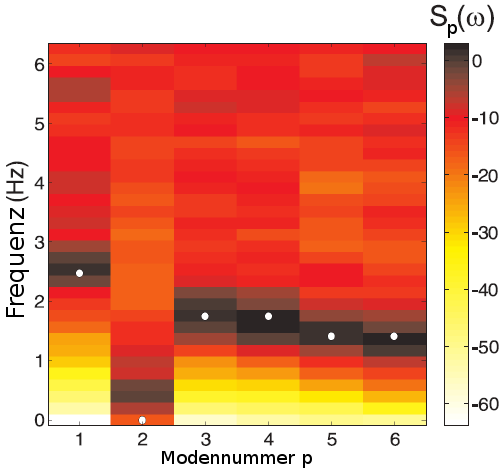
\includegraphics[width=\textwidth,height=0.3\textheight]{figs/modenvenergie3teilchenmelzer.png}
								\caption{}
								\label{img:spektrum}
							\end{subfigure}
							\begin{subfigure}[b]{0.48\textwidth}
								\centering
								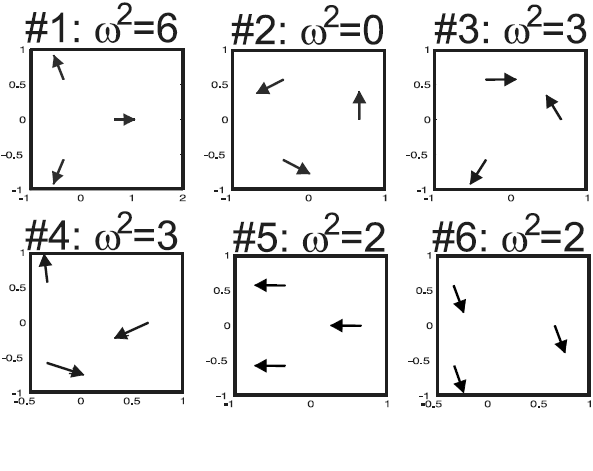
\includegraphics[width=\textwidth,height=0.3\textheight]{figs/modenvektoren3teilchenmelzer.png}
								\caption{}
								\label{img:moden}
							\end{subfigure}
							\caption{\fett{(a)}: Modenspektrum für einen 3-Teilchen-Cluster. Die weißen Punkte entsprechen theoretisch errechneten Werten der Modenfrequenzen. Die Bereiche von $S\ix{p}\left(\omega\right)\rightarrow0$ treten bei der Eigenfrequenz auf. \fett{(b)}: Eigenvektoren ($\vec{\nu}\ix{i,p}$) für $N=3$. Die Modenfrequenz ist auf die Einfangstärke $\omega\ix{0}$ normiert (nach \cite{Melzer12}).}
						\end{figure}

					Die spektrale Energiedichte aus Gl. (\ref{eq:energiedicht}) wird in \ref{img:spektrum} für einen sehr simplen Cluster aus $N=3$ Teilchen dargestellt. Passend dazu sind in \ref{img:moden} die Modenvektoren der drei Staubpartikel eingezeichnet. Insbesondere sind dort Moden gezeigt, welche allgemein für alle Cluster auftreten: \tilt{breathing}, \tilt{slosh} und Rotation. $p=1$ zeigt die \tilt{breathing}-Mode: alle Teilchen entfernen sich vom Clusterschwerpunkt, wobei dieser jedoch fest bleibt. Die Frequenz $\omega\ix{breath}$ hängt schwach von $N$ ab und steigt mit der Abschirmung $\kappa$. Mode $p=2$ ist die Rotationsmode. Ihre Eigenfrequenz ist $0$, da es für diese keine rückstellenden Kräfte gibt. In $p=3$ und $p=4$ sind \tilt{kink}-Moden gezeigt. Nummer 5 und 6 stellen \tilt{slosh}-Moden dar: das System führt eine Schwerpunktstranslation aus, wobei alle Partikel sich in die selbe Richtung bewegen.\\
					Diese \tilt{Normalmodenanalyse} ist ein geeignetes Mitte zur Analyse der Dynamik eines finiten Systems (siehe \cite{Melzer01},\cite{Melzer03}), vorausgesetztes genügt den gemachten Voraussetzungen: Yukawa-Wechselwirkung, starke Kopplung jedoch fluider Zustand, homogene Partikel \dots

				\subsubsection*{Fluidmoden}

					Genau wie in der, diesem Teilgebiet übergeordneten Plasmaphysik, lässt sich ein finiter Cluster als hydrodynamische Gesamtheit auffassen. Ähnlich wie beim \tilt{Fluidmodell} und der Betrachtung durch die \tilt{magnetohydrodynamischen Gleichugen} (MHD), nimmt man hierbei das System als kontinuierliche Masse mit entsprechender Ladungsverteilung an. Daraus ergeben sich neue Möglichkeiten die Dynamik des Cluster zu beschreiben und nachzuvollziehen.\\
					Eingangs muss das neue Potential $\Phi\left(\vec{r},t\right)$ des fluiden "`Tropfens"' beschrieben werden. Da der Cluster von Ladungsträgern abgeschirmt wird, welche sich um diesen auf Grund seiner elektrostatischen Wechselwirkung ansammeln - analog zu den vorherigen Abschnitten -, kann man die modifizierte Poissongleichung (Gl. (\ref{eq:poisson})) für die Ladungsdichte $\rho\left(\vec{r},t\right)$ des Systems benutzen. Deren Lösung erhält man mit der \tilt{Green-Funktion} $G\left(\vec{r}\right)$ aus Gl. (\ref{eq:green}) in (\ref{eq:fluid}). 

						\begin{align}
							&\left(\Delta-\kappa^2\right)\Phi\left(\vec{r},t\right)=\frac{1}{\varepsilon\ix{0}}\rho\left(\vec{r},t\right) \label{eq:poisson} \\
							\Phi\left(\vec{r}\right)&=\int_{\mathbb{R}^3}\frac{\rho\left(\vec{r}\,^\prime,t\right)}{4\pi\varepsilon\ix{0}|\vec{r}-\vec{r}\,^\prime|}\diff^{3}r^\prime \\
							&\,\,\,\,\vdots\quad G\left(\vec{r}\right)=\frac{\exp\left(-\kappa|\vec{r}|\right)}{4\pi|\vec{r}|} \label{eq:green}\\
							\Phi\left(\vec{r}\right)&=\int_{\mathbb{R}^3}\frac{\exp\left(-\kappa|\vec{r}-\vec{r}\,^\prime|\right)}{4\pi\varepsilon\ix{0}|\vec{r}-\vec{r}\,^\prime|}\rho\left(\vec{r}\,^\prime,t\right)\diff^{3}r^\prime \label{eq:fluid}
						\end{align}

					Die Green-Funktion entspricht einem einheitenlosen Yukawa-Potential, welches man nach \cite{Arfken05},\cite{Yap10} in eine Reihe von sphärisch-harmonischen \tilt{Kugelflächenfunktionen} $Y_{lm}\left(\theta,\varphi\right)$ und \tilt{modifizierten Besselfunktionen} $i_{l}\left(x\right)$ und $k_{l}\left(x\right)$ entwickeln kann. Die Definitionen erfolgen in dreidimensionalen Kugelkoordinaten $\left(r,\theta,\varphi\right)$, wobei die minimalen bzw. maximalen Abstände $r\ix{<}=\min\left(r^\prime,r\right)$ und $r\ix{>}=\max\left(r^\prime,r\right)$ sind.

						\begin{align}
							\frac{\exp\left(-\kappa|\vec{r}-\vec{r}\,^\prime|\right)}{4\pi|\vec{r}-\vec{r}\,^\prime|}=\sum_{l=0}^{\infty}\sum_{m=-l}^{l}\frac{r\ix{<}^l}{r\ix{>}^{l+1}}i_{l}\left(\kappa r\ix{<}\right)k_{l}\left(\kappa r\ix{>}\right)\exp\left(-\kappa r\ix{>}\right)Y_{lm}^*\left(\theta^\prime,\varphi\prime\right)Y_{lm}\left(\theta,\varphi\right) \label{eq:entwick}
						\end{align}

					Nach \cite{Ivanov09} und \cite{Schella13} lassen sich aus Gl. (\ref{eq:entwick}) die Multipolmomente der Ladungsdichte des Clusters gewinnen (siehe Gl. (\ref{eq:multipol})). Die Indizes $lm$ geben die Modenzahlen an, wobei analog zu den Zust\"anden eines Wasserstoff-artigen Atoms $\Psi\left(\vec{r}\right)=L_{n}\left(r\right)Y_{lm}\left(\theta,\varphi\right)$ diese die Symmetriezahlen bzw. -richtungen der Schwingungen des Staubtropfens angeben (siehe \ref{img:fluidmode}).

						\begin{align}
							\rho_{lm}\left(t\right)=&\sqrt{\frac{4\pi}{2l+1}}\int_{\mathbb{R}^{3}}\rho\left(\vec{r},t\right)i_{l}\left(\kappa r\right)Y^{*}_{lm}\left(\theta,\varphi\right)\diff^{3}r \label{eq:multipol} \\
							Q_{lm}\left(\omega\right)=&\left.\left.\frac{2}{TN}\right|\int_{0}^{T}\rho_{lm}\left(t\right)\exp\left(-\imag\omega t\right)\diff t\right|^{2}
						\end{align}

					Wie in Gl. (\ref{eq:energiedicht}) wird \"uber die Fouriertransformation aus dem Zeit- in den Frequenzraum die anteilige Energie der Mode $q_{lm}$ an der Schwingungsbewegung des Tropfens bei $\omega$ in der korrespondierenden Periode  $T$ berechnet. Das Frequenzpektrum stellt somit die Zusammensetzung der Clusterbewegung aus den Moden $lm$ dar.\\
					Nach Gl. (\ref{eq:multipol}) k\"onnen die einzelnen Moden als Dipol, Quadrupol, \dots identifiziert werden. Ihren Symmetriezahlen $lm$ entsprechend, vollf\"uhrt der Cluster dabei die bereits bekannten Schwingungen (siehe \ref{subsub:moden}): die \tilt{breathing}- und \tilt{slosh}-Mode. Dabei ist das Tupel $\left(l=0,m=0\right)$ die Monopolschwingung: eine periodischen Kompression und Relaxation des Systems (\tilt{breathing}). Die Indizes $\left(l=0,m=1\right)$ und deren Permutation stellen eine Dipolschwingung dar. Der Ball vollf\"uhrt eine Schwerpunktstranslation (\tilt{slosh}). Die Beschreibung einer Rotationsbewegung fehlt, da die Ladungsverteilung invariant gegen\"uber Drehungen ist. H\"ohere Symmetrien - Schwingungen auf 2 oder mehr Raumachsen - entsprechen demnach h\"oheren Werten von $\left(l,m\right)$. Die in diesem Versuch betrachteten Bewegungen sind Quadrupol- bzw. Hexapolschwingungen.

						\begin{figure}[H]
                            \centering
                            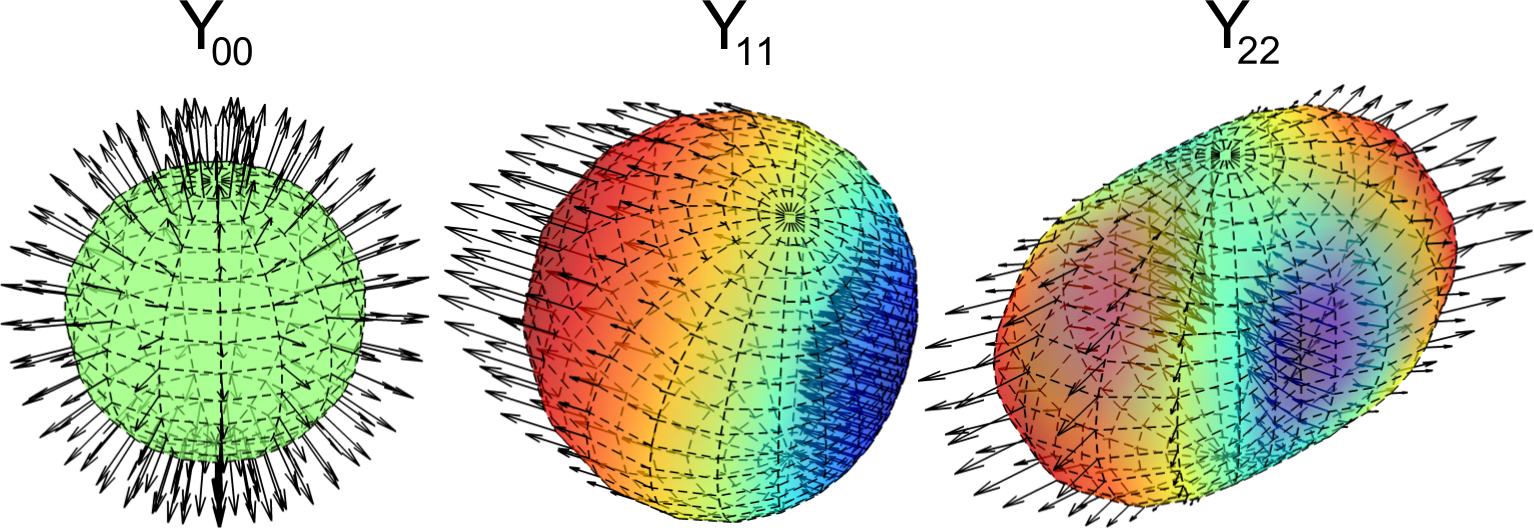
\includegraphics[width=\textwidth,height=0.375\textwidth]{figs/y001122.png}
                            \caption{Darstellung der Fluidmoden über Kugelflächenfunktionen mit Pfeilen als charakteristische Schwingungsrichtungen bzw. -achsen. Rote Bereiche sind als Regionen hoher Dichten, blaue als jene niedrigerer zu interpretieren. Von links nach rechts: Monopol (\tilt{breathing}), Dipol (\tilt{slosh}), Quadrupol (nach \cite{Mulsow13}).}
                            \label{img:fluidmode}
                        \end{figure}

	\newpage

	\section{Durchführung}\label{sec:durch}

		Im anschlie{\ss}nende Abschnitt wird der Aufbau, sowie die Durchf\"uhrung und die Messmethodik des Experiments dieser Arbeit umrissen. Es folgt eine Beschreibung der Plasmakammer, sozusagen als Vertiefung des Abschnitts \ref{sub:kaprfplasm}, einschlie{\ss}lich der Kameraanordnung mit Beleuchtungslasern. Eine Betrachtung des sog. \tilt{Plasma-Glow} wird ebenso Teil dieses Abschnitts sein. Zus\"atzlich soll dabei die dreidimensionale Rekonstruktion der Partikelbewegungen aus den Kamerabildern kurz beschrieben werden.

			\begin{figure}[H]
				\centering
				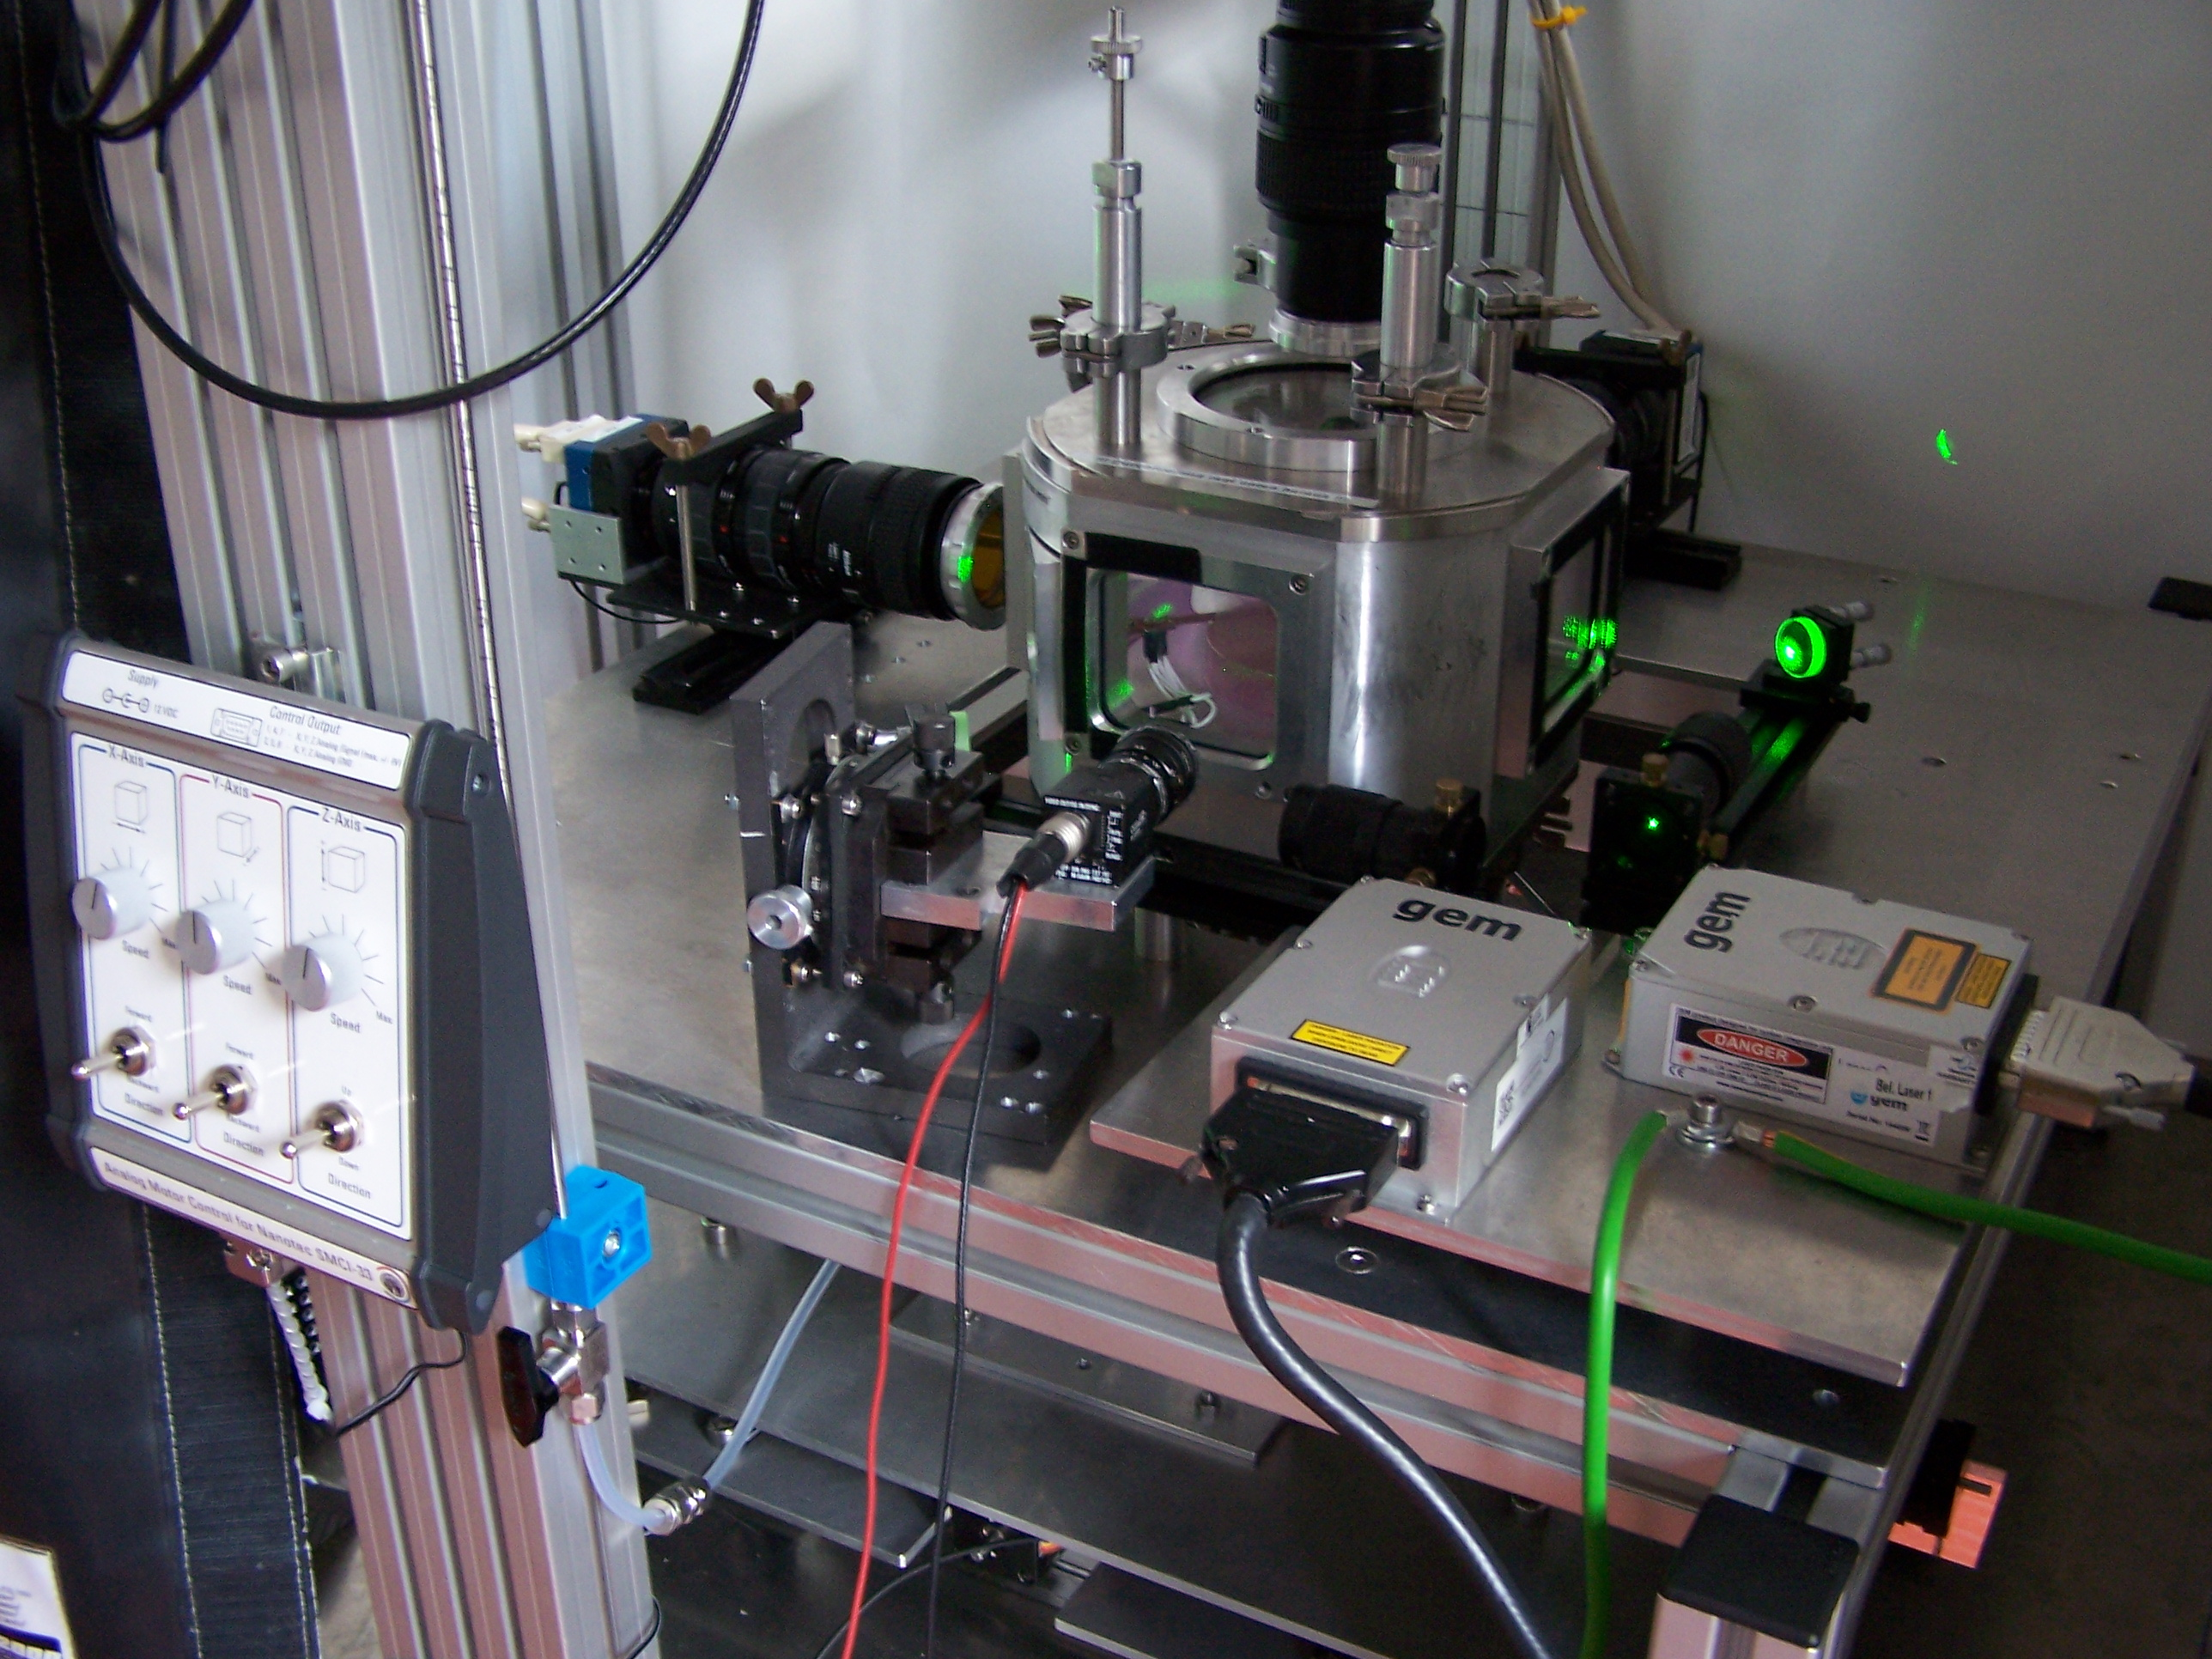
\includegraphics[width=\textwidth,height=0.7\textwidth]{figs/cam/aufbau.jpg}
				\caption{Photografierter, vollständiger Versuchsaufbau bei eingeschaltetem Plasma mit grünen Beleuchtungslasern und verschiebbarem Tisch (siehe Steuerung links). Eine kleine Schwarz-Weiß-Übersichtskamera (Bildmitte vor der Kammer) ermöglichte auch bei laufendem Experiment die Beobachtung des Kammerinneren. Um den Versuch herum befand sich, als Sicherheitsvorkehrung, ein Laserschutzvorhang (Hintergrund).}
				\label{img:photo}
			\end{figure}

		\subsection{Aufbau}

			Die in diesem Experiment verwendete Plasmakammer wird in \ref{img:plasmakammer} gezeigt. Den fertigen Aufbau, samt Beleuchtungslaser und elektrisch verschiebbaren Versuchstisch zeigt das Photo in \ref{img:photo}. Die Kammer hat einen Innendurchmesser von $\unit[25]{cm}$, wobei deren W\"ande sowie Boden aus Aluminium und der Deckel aus Edelstahl besteht. Vier gro{\ss}e und 2 kleine, seitlich angebrachte, antireflexbeschichtete Fenster erm\"oglichen 2 der 3 Kameras aus der Ebene den Blick auf den Yukawa-Ball. Im Deckel der Kammer befindet sich ein kreisrundes, etwa $\unit[9]{cm}$ im Durchmesser gro{\ss}es Fenster f\"ur die letzte Kamera, welche orthogonal zu den \"ubrigen angebracht ist. Dieses stereoskopische System nutzt man letztendlich zur Rekonstruktion der Teilchentrajektorien in 3D.


       			\begin{figure}[t]
       				\centering
       				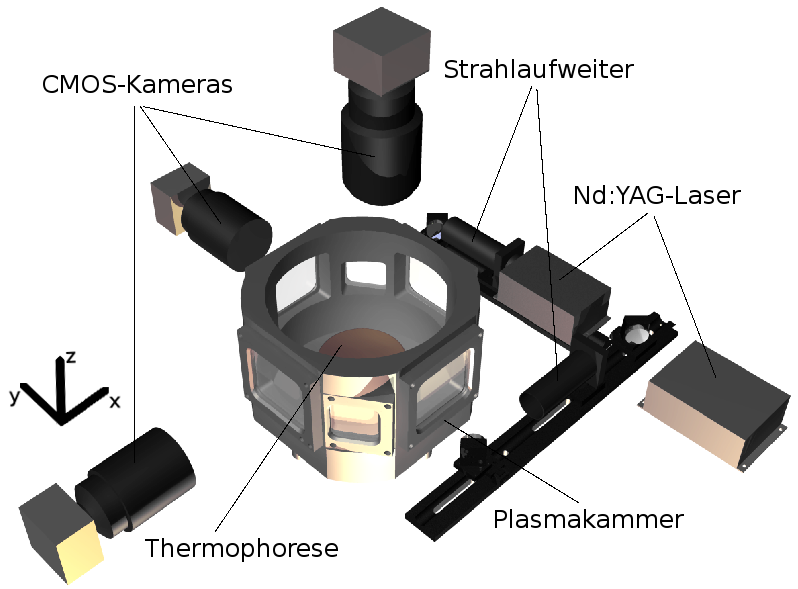
\includegraphics[width=0.75\textwidth,height=0.55\textwidth]{figs/witharrowsnunu.png}
       				\caption{Perspektivische Ansicht eines Schemas des Aufbaus aus \ref{img:photo}. Das eingezeichnete Koordinatensystem (rechts unten) entspricht dem der Tischbewegung und der späteren Auswertung (nach \cite{Mulsow13}).}
       				\label{img:plasmakammer}
       			\end{figure}

			Wie im Abschnitt \ref{sub:kaprfplasm} beschrieben, wird in diesem Versuch ein kapazitiv gekoppeltes Niederdruck-Radiofrequenz-Plasma in einer asymmetrischen Entladungskammer erzeugt. Eine abgeschirmte Messingelektrode befindet sich im unteren Teil des Aufbaus und wird, \"uber die besprochene kapazitive Kopplung zur Anpassung von Gleistromanteilen, von einem Radiofrequenz-Generator mit einer Leistung zwischen $\unit[1-3]{W}$ und bei einer Frequenz von $\unit[13,56]{MHz}$ betrieben. Der \"ubrige Teil der Begrenzung liegt auf Massepotential und dient damit als, fl\"achenm\"a{\ss}ig um ein vielfaches gr\"o{\ss}ere Gegenelektrode. \"Uber eine Pumpe wird die Kammer bis auf einen Restdruck von etwa $\unit[\tenpo{-1}]{Pa}$ evakuiert, damit sie m\"oglichst frei von Umgebungsluft ist und anschlie{\ss}end eine reine Argon-Entladung bei $\unit[5-12]{Pa}$ erzeugt werden kann.
			Weiterhin befinden sich im Deckel der Kammer Durchf\"uhrungen f\"ur den Staub aus MF (Melamin-Formaldehy) - $\unit[4,86\pm0,07]{\mu m}$ im Radius - und die Einfang-Elektrode. Die Partikel werden \"uber ein Reservoir der Gr\"o{\ss}e eines 1 Cent-St\"uckes mit einer $\unit{\mu m}$-gro{\ss}en Bohrung in die Entladung eingebracht. Die Befestigung der Ringelektrode aus \ref{img:eingefangenerball} ist h\"ohenverstellbar und l\"asst sich leicht drehen, damit eine optimale Positionierung des Cluster in der Randschicht \"uber der getriebenen Elektrode bzw. der geheizten Thermophorese vorgenommen werden kann. Letztere liegt auf der unteren Elektrode auf und ist \"uber Vakuumschl\"auche und einen Einsatz in der Kamerwand mit einem Wasserbad au{\ss}erhalb verbunden.

    			\begin{figure}[t]
    				\begin{subfigure}[t]{0.48\textwidth}
    					\centering
    					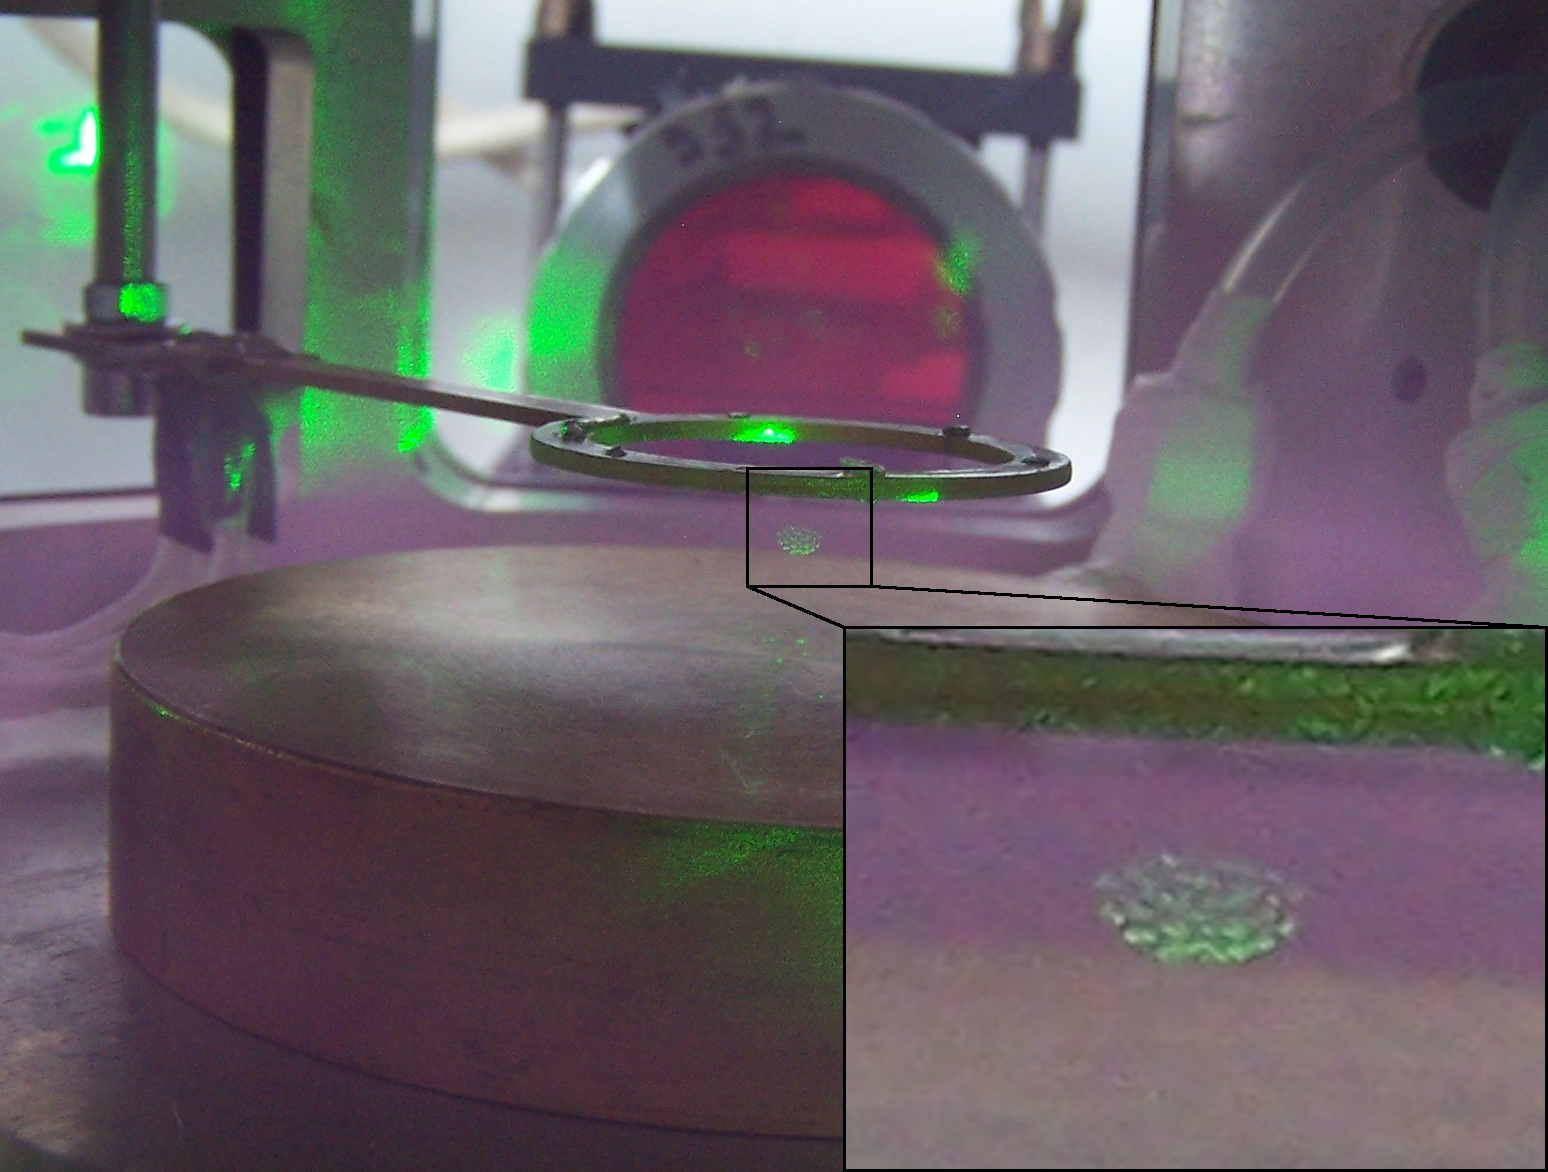
\includegraphics[width=\textwidth,height=0.75\textwidth]{figs/cam/innenansicht.jpg}
    					\caption{}
    					\label{img:eingefangenerball}
    				\end{subfigure}
    				\begin{subfigure}[t]{0.48\textwidth}
    					\centering
    					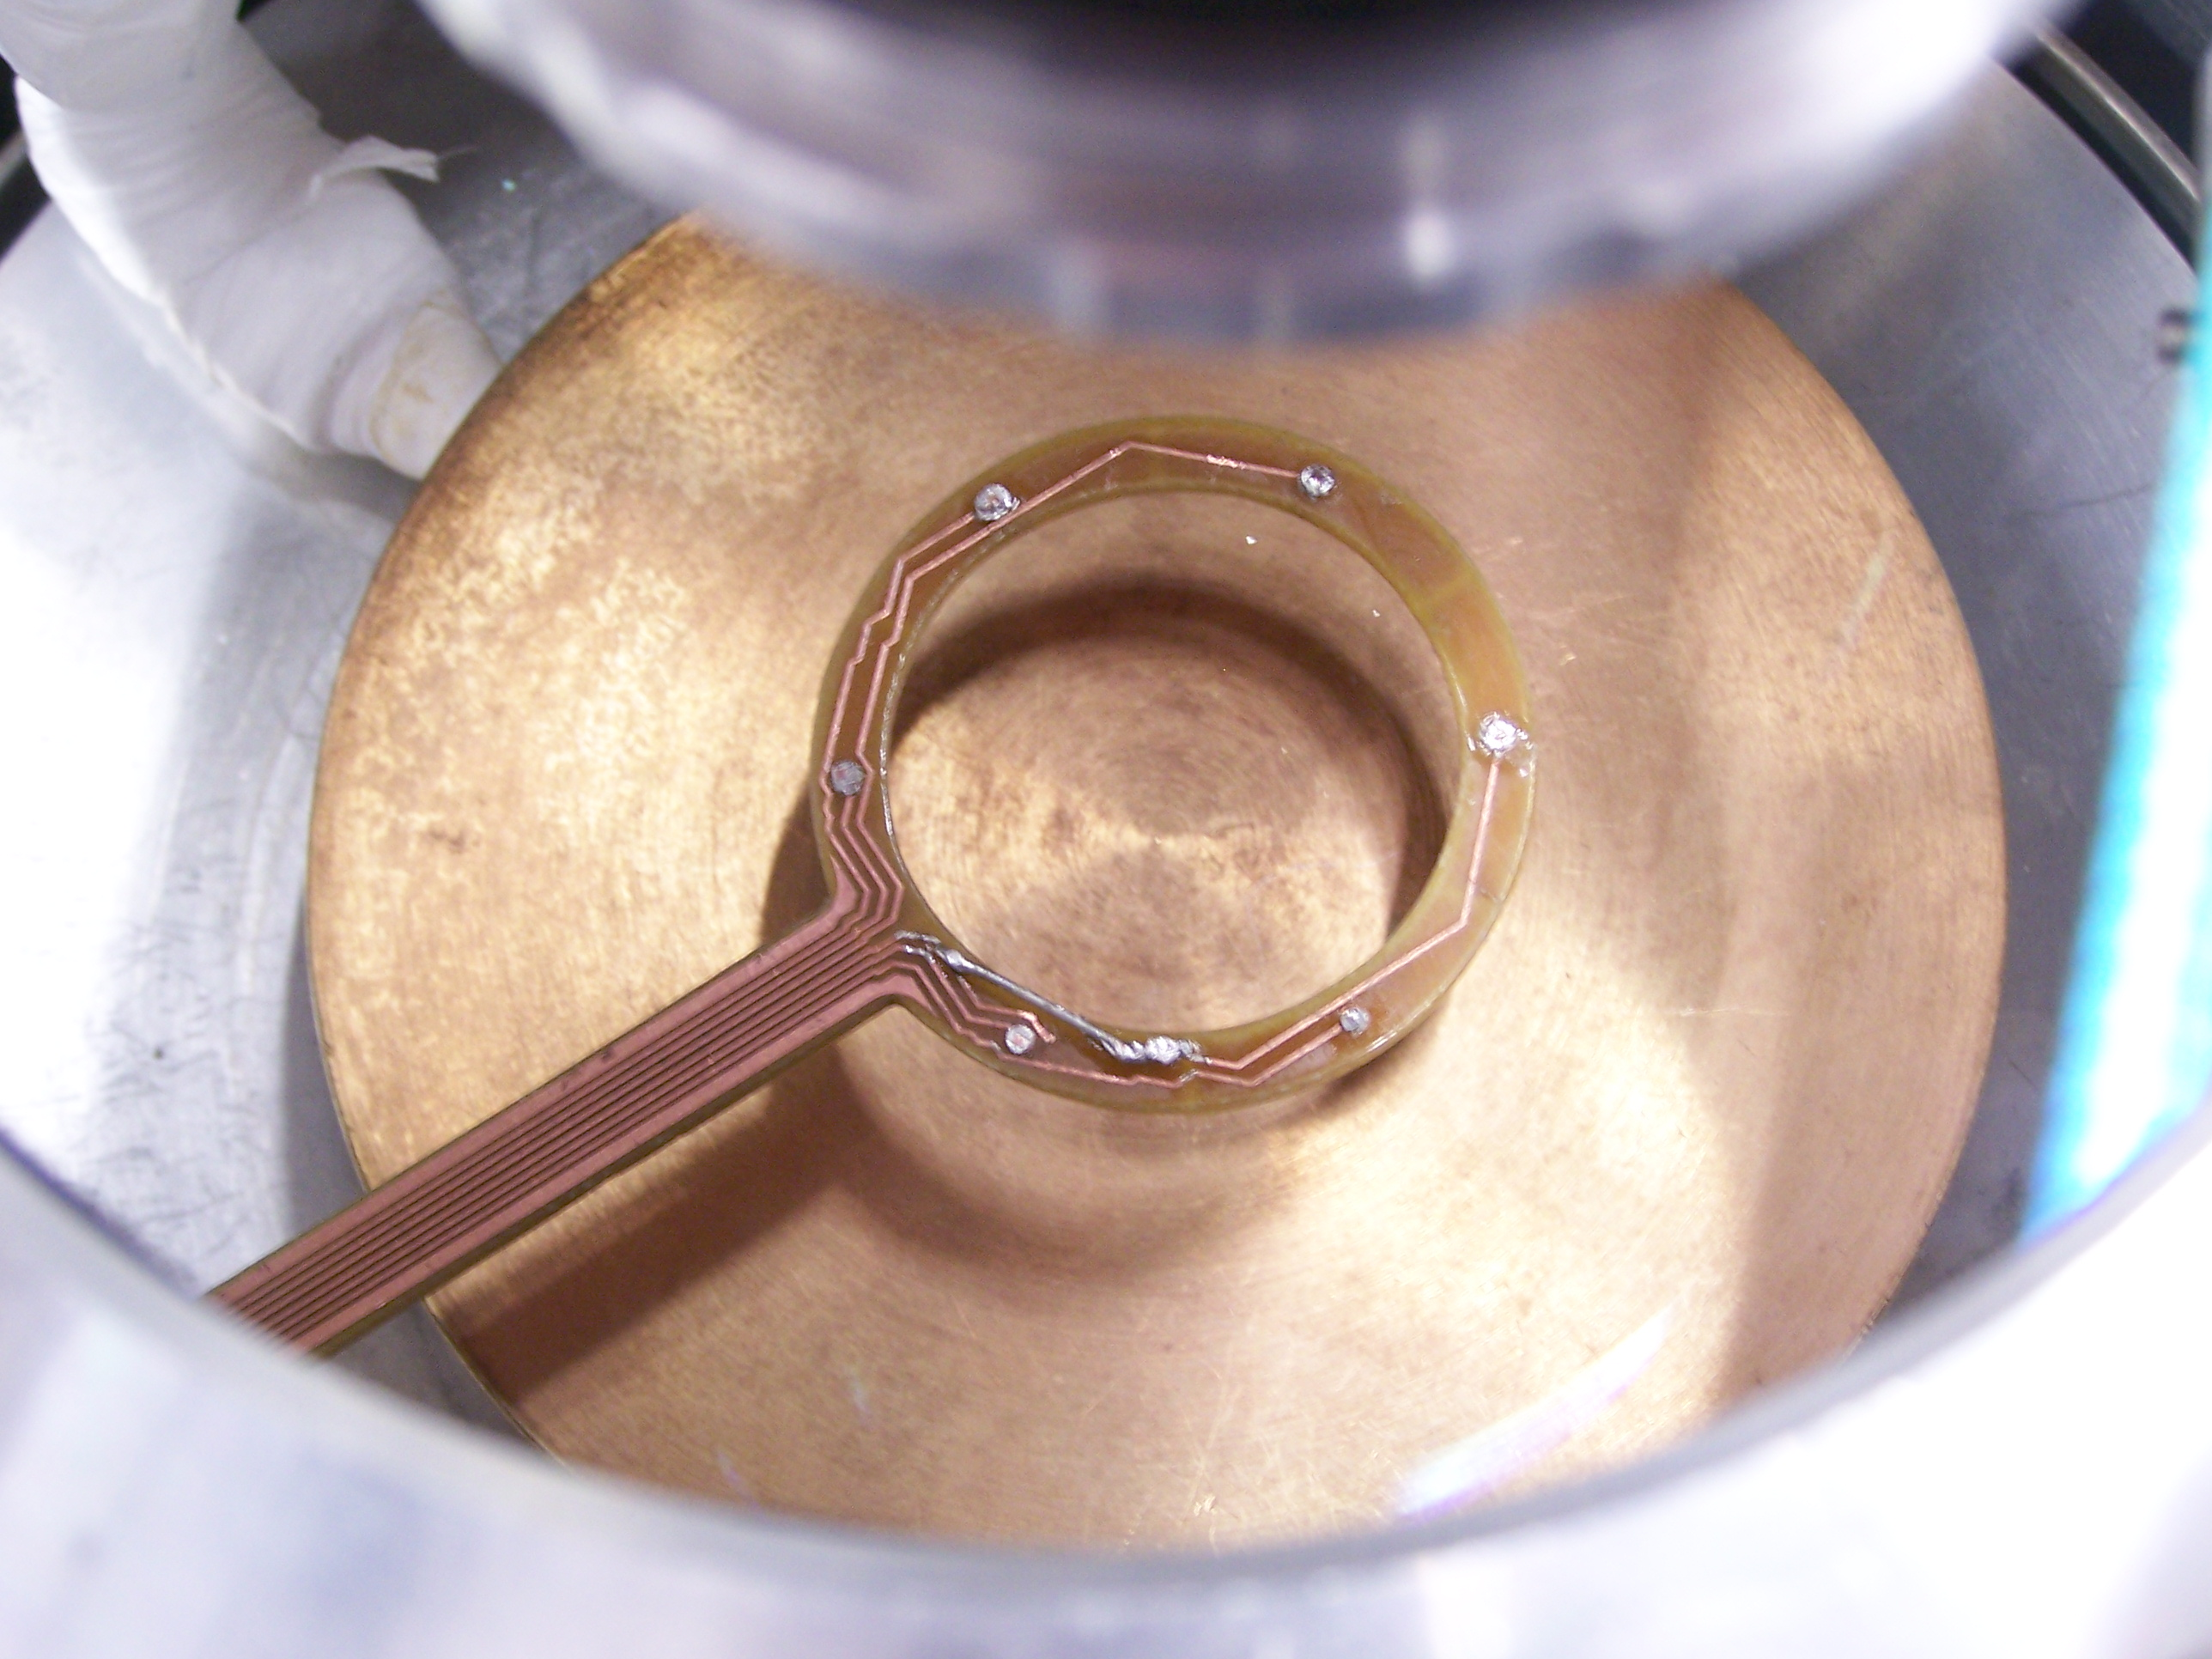
\includegraphics[width=\textwidth,height=0.75\textwidth]{figs/cam/topview.jpg}
    					\caption{}
    					\label{img:topview}
    				\end{subfigure}
    				\caption{\fett{(a)}: Einfang eines Yukawa-Balls mit $N\approx40$ unter Beleuchtung mit Nd:YAG-Lasern. Der Cluster befindet sich, leicht abhängig von der Höhe des Rings in der Randschicht, circa $\unit[0,5-1]{cm} $ unterhalb der Elektrode. Im Hintergrund: Kamera 'rot' mit Filter für $\unit[532]{nm}$. \fett{(b)}: Draufsicht durch den Deckel der Kammer auf den Ring. Günstiger Weise befindet sich dieser in der Mitte der Thermophorese, damit aus Sicht des, relativ dazu kleinen Clusters, die Randschicht unendlich ausgedehnt ist.}
    			\end{figure}

			Die für den Einfang der Cluster genutzten Segmentringe - wie der in \ref{img:ring} aus Abschnitt \ref{sub:einfang} - sind \"uber Kabel mit Abschirmung und eine weitere, unten liegende Vakuum-Durchf\"uhrung (4- bzw. 8-polig) mit der Manipulationselektronik verbunden. Das erm\"oglicht es, verschiedenste Signale auf die einzelnen Bereiche der Elektrode zu bringen und damit das System gezielt zu heizen bzw. Moden anzuregen (siehe \ref{img:ring}). Um den Ring, welcher als Antenne im Plasma fungiert, pr\"aziser abstimmen zu können, wurde ein Trimmnetzwerk zwischen analogem Ausgang der Anregung und Elektrode geschaltet. Mittels Potentiometern und einem zus\"atzlichen Netzteil k\"onnen so gr\"o{\ss}ere Potentiale mit erh\"ohter Genauigkeit angelegt werden.

		\subsection{Elektrischer Einfang} \label{sub:einfang}

				\begin{wrapfigure}{r}{0.5\textwidth}
					\centering
					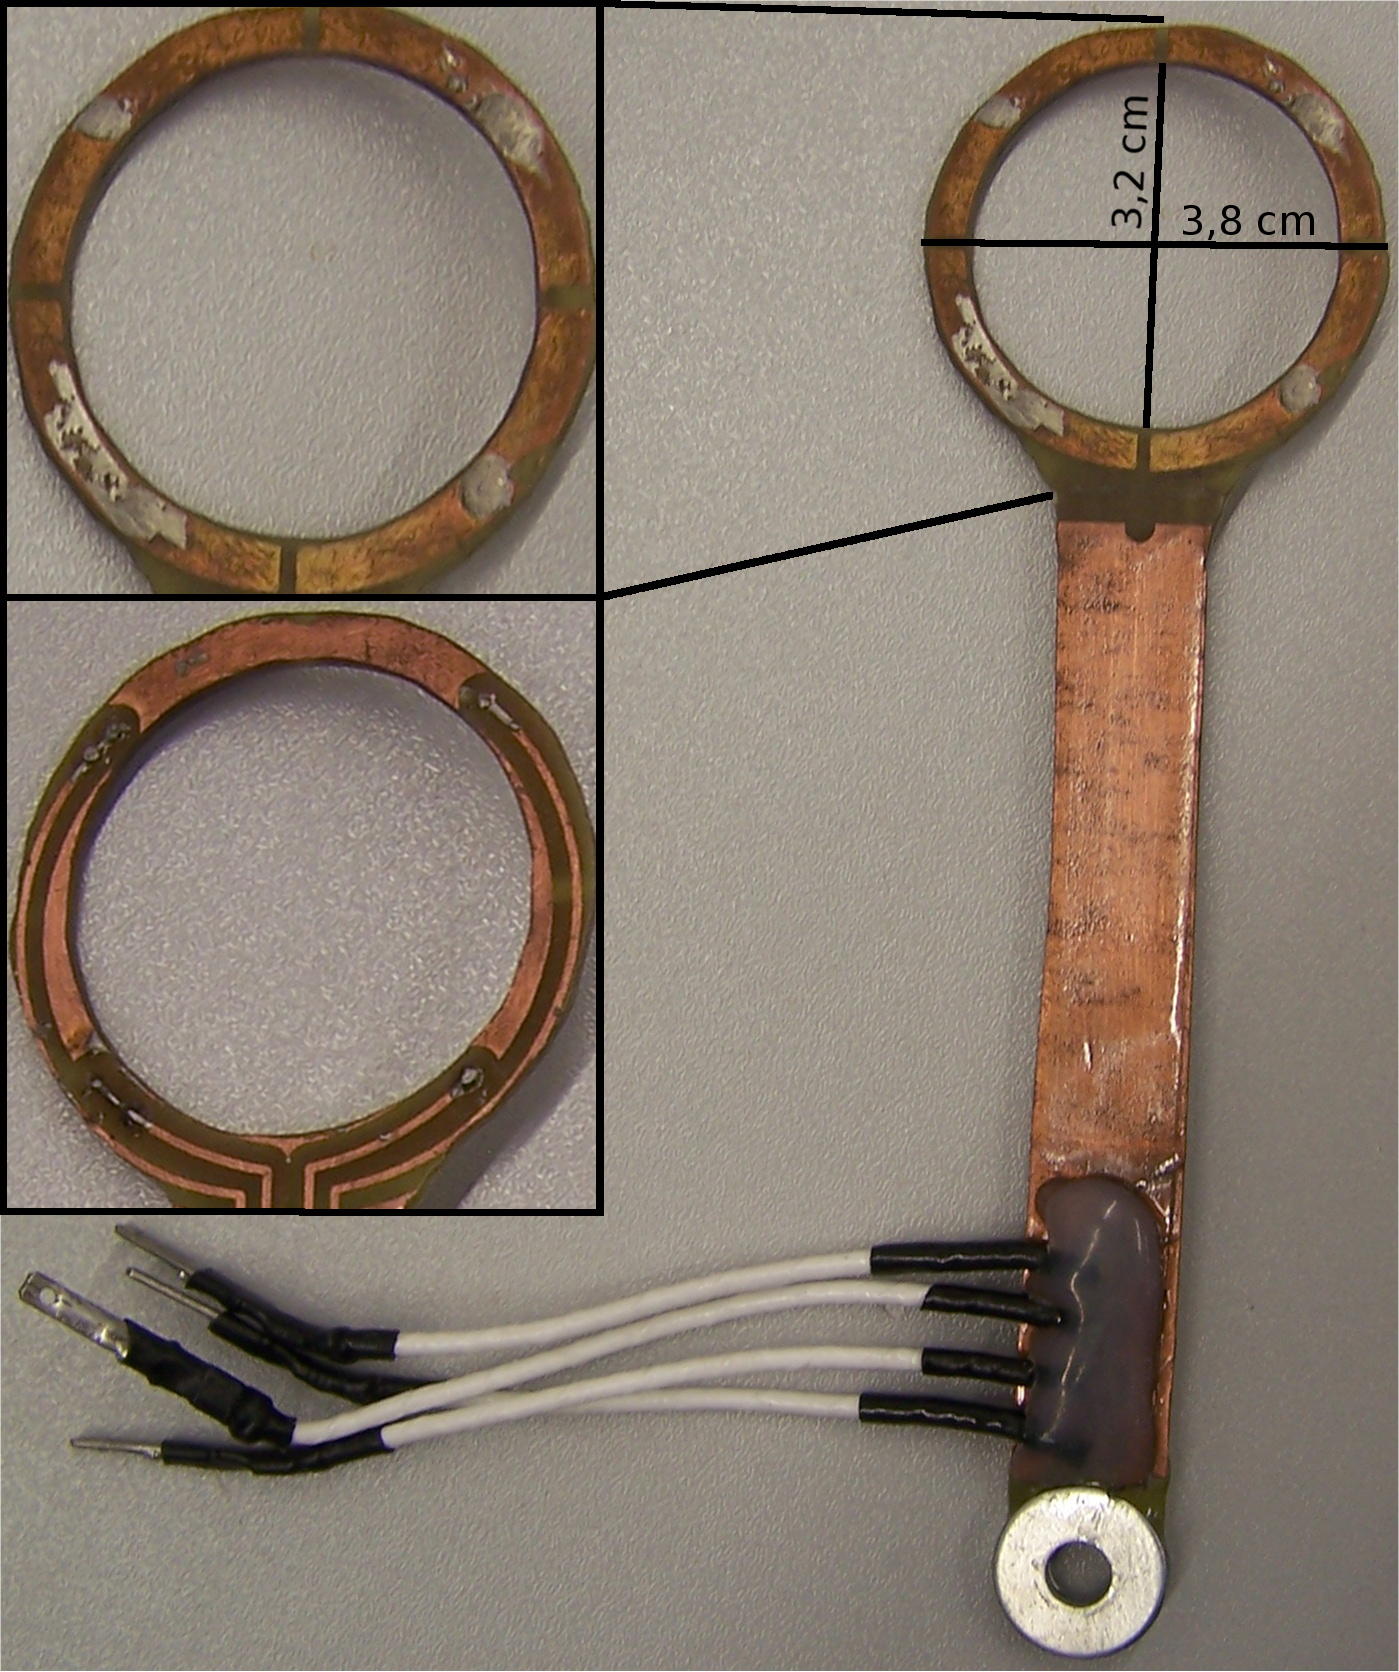
\includegraphics[width=0.45\textwidth,height=0.55\textwidth]{figs/cam/ringelektrode.jpg}
					\caption{4-segmentiger Kupferring \underline{nach} der Benutzung. Es zeigen sich trotz Schutz durch Plastikumhüllung starke Abnutzungen durch das \tilt{sputtering}. Am unteren Ende sind die weißen Vakuumkabel zu sehen.}
					\label{img:ring}
				\end{wrapfigure}

			Hauptaugenmerk dieses Experiments ist die Manipulation der Randschicht des Plasmas \"uber der getriebenen Elektrode und finiter Yukawa-Systeme. Hierf\"ur wurden eigens mehrsegmentige Kupferplatinen konzipiert und konstruiert, siehe \ref{img:ring}. Deren globaler (auf Skalen des Clusters) Einflu{\ss} auf die Randschicht erm\"oglicht den Einfang eines Staubballs bei niedrigen Gasdr\"ucken und Plasmaleistungen. Weiterhin ist die Geometrie der Ringelektrode besonders g\"unstig f\"ur das vorliegende System, da sich somit ein sehr homogenes, sich der Symmetrie des Clusters angepasstes Einfangpotential einstellt.\\
			Prinzipiell bestehen die verwendeten Elektroden aus einem $\unit[6]{mm}$ starken, $\unit[3,2]{cm}$ im Inneren messenden Ring mit 4,6 oder 8 Segmenten aus Kupfer an der Unterseite, welche später in Richtung des Clusters in der Randschicht zeigen. Dieser Ring ist mit einem Arm, über den die Leiterbahnen der jeweiligen Segmente laufen, verbunden. Am Ende dessen befindet sich eine Bohrung, durch welche die Durchführung mit Schraubgewinde im Kammerdeckel geführt werden kann und somit die Positionierung bei geschlossenem Aufbau ermöglicht. Die gelöteten Kontaktierungen der Vakuumkabel für die Manipulation, von der Ober- auf die Unterseite führend, liegen knapp vor der Bohrung. Für einen Vergleich siehe \ref{img:ring}.\\
			Ziel der Manipulation durch die segmentierte Ringelektrode ist es, verschiedene Moden mit unterschiedlichen Symmetrien - zweizählig für Dipol, 4 zählig für Quadrupol usw. - gezielt anzuregen und in diese Energie zu bringen. Durch die Modentheorien aus Abschnitt  \ref{sub:yukawaclust} und deren Ausdrücke für die Energie pro Mode $Q_lm\left(\omega\right)$ bzw. $S\ix{p}\left(\omega\right)$ kann danach bestimmt werden, inwiefern die Störung erfolgreich war und welche Konsequenz dies nach sich zieht. Auf die Veränderung der Randschicht durch den Ring wird in \ref{sub:glow} eingegangen.


		\subsection{Strereoskopie und Bildrekonstruktion}

			Die Skala der Dynamik der Staubteilchen bzw. des Plasma-Glow erlauben eine strereoskopische Untersuchung des Systems. Die Beobachtung erfolgte \"uber 3, zueinander orthogonale High-Speed-CMOS-Kameras mit 60 bzw. $\unit[105]{mm}$ Objektiven. Deren Aufnahmen von bis zu 500 Bildern pro Sekunde ($\unit{fps}$ - \tilt{frames per second}) haben eine maximale Aufl\"osung von $\unit[1280x1024]{px}$. Dabei nimmt die \tilt{fps}-Zahl stark mit steigender Auflösung ab: je mehr Daten aufgenommen und verarbeitet werden müssen, umso niedriger ist die maximale, verlustfreie Aufnahmerate.\\
			Für die Messreihen wurden jeweils Bilderserien von 10000 \tilt{frames} aufgenommen, wobei die Geschwindigkeit sich dem zu untersuchenden Sachverhalt anpasste. F\"ur eine "`freie"' Aufnahme lag diese bei 100 Bildern pro Sekunde: der Cluster war entweder ungest\"ort oder wurde bei einer festen Anregungsfrequenz manipuliert. Waren Informationen zu bestimmten Phasen gesucht, so wurde dementsprechend die Kamera mit der Anregung gekoppelt und dabei 4 Bilder pro Periode bei einer Frequenz von bis zu $\unit[6,5]{Hz}$ gemacht. \\
			Beleuchtet wurde der Yukawa-Ball mit 2 gr\"unen Nd:YAG-Lasern, welche bei einer Wellenl\"ange von $\unit[532]{nm}$ und mit einer Leistung von $\unit[600]{mW}$ abstrahlten. Über Strahlaufweiter und Spiegel wurden die Laser diagonal durch die Entladung geleitet (siehe \ref{img:eingefangenerball}). Strahlprofil und Strahlungsdruck (siehe \ref{subsub:laser}) sind durch diesen Aufbau so konstruiert, dass sie f\"ur die Dynamik des Clusters unkritisch sind.\\
			Da die Ausdehnung der Partikel weniger als $10\cdot\lambda$ des Laserlichts ist (siehe \cite{Mie08} o. \cite{Hulst81}), kann zur Beschreibung des Streuverhaltens der Staubteilchen die Mie-Streuung herangezogen werden (\cite{Bonitz10}). Nach dieser Theorie ist das vorw\"arts gestreute Licht, nach dem reflektierten, am intensivsten. Deswegen befinden sich die Kameras auf den gegen\"uberliegenden Seiten der Punkte, an denen das Laserlicht eingestrahlt wird: es resultiert ein kontrastreiches Bild, auf welchem die Partikel gut vor dem dunklen Hintergrund zu sehen sind (siehe \ref{img:rechts} und weitere). Damit einher gehen jedoch auch Probleme, wie zBsp. das es zu einer \"Uberbelichtung oder Komplikation bei der Ausrichtung des Systems aus Cluster, Elektrode, Laser und Vakuumkabel kommen kann.\\
			Die Bildverarbeitung erfolgte im graustufigen \tilt{device-independent-bitmap}-Format, kurz \tilt{*.bmp}. Dabei handelt es sich um ein zweidimensionales Rastergrafikformat, bei dem, wie in einer Matrix mit jeweils 3 Elementen je Zelle, einem Pixel die RGB-Informationen mit insgesamt 3 8-Bit-Werten zugeordnet werden. Das erleichterte u.a. die Verarbeitung in Hinblick auf Intensit\"atsanalysen, wie die Partikelerkennung oder die Auswertung des Plasma-Glow (siehe \ref{sub:glow}).
            
                \begin{figure}
                    \begin{subfigure}[b]{0.4\textwidth}
                        \centering
                        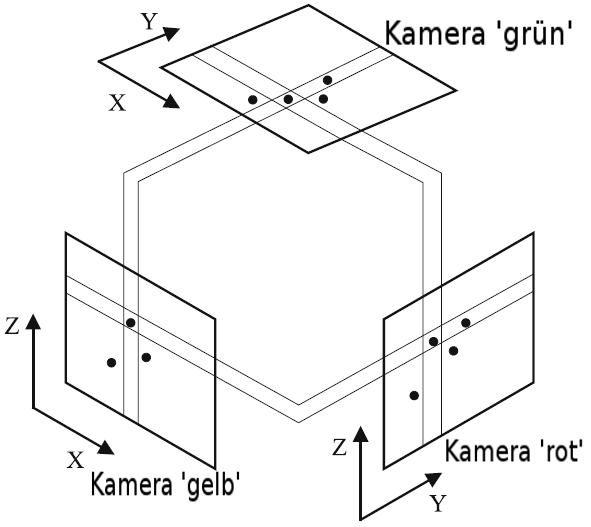
\includegraphics[width=\textwidth,height=5.5cm]{figs/rekonstruktion.png}
                        \caption{}
                    \end{subfigure}
                    \begin{subfigure}[b]{0.56\textwidth}
                        \centering
                        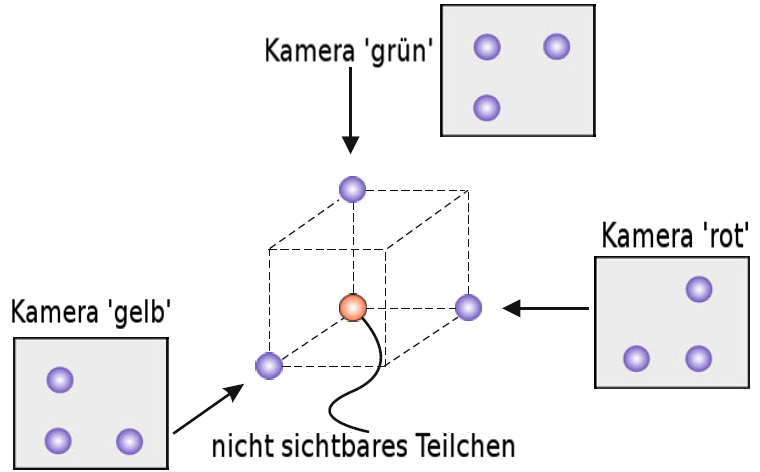
\includegraphics[width=\textwidth,height=5.5cm]{figs/nichtsichtbar.png}
                        \caption{}
                    \end{subfigure}
                    \caption{\fett{(a)}: Rekonstruktion der dreidimensionalen Informationen aus den Bildern der Kameras. \fett{(b)}: Fehler in der Analyse durch Überlagerung von 4 Teilchen in drei Bildern. Für kurze Zeiten des 'Verschwindens' kann mittels Interpolation die Trajektorie des nicht sichtbaren Teilchens vervollständigt werden (nach \cite{Bonitz10}).}
                    \label{img:rekonstruktion}
                \end{figure}

				\subsubsection{3D-Trajektorien}

					Die Rekonstruktion der dreidimensionalen Informationen des Beobachtungsvolumen ist das Kernst\"uck der Stereoskopie (\cite{Bonitz10}). Eingangs m\"ussen aus den einzelnen \tilt{frames} der Kameras die Partikelpositionen gewonnen werden. Daf\"ur analysiert man das Bild durch einen (\tilt{gau{\ss}schen}) Bandpass der Breite des erwarteten Partikeldurchmessers (\cite{Crocker96a}, \cite{Ivanov07}). Au{\ss}erhalb liegende Objekte werden gegl\"attet und angepasst. F\"ur alle erkannten Teilchen wird anschlie{\ss}end, der Intensit\"atsverteilung \"uber diese entsprechend, deren Schwerpunkt ermittelt. Daraus erh\"alt man f\"ur alle Kameras die zweidimensionalen Informationen \"uber Partikelpositionen und Clusterausdehnung.\\
					Die Zuordnung der Partikel in gleichzeitigen Kamera-\tilt{frames} ist in \ref{img:rekonstruktion} schematisch dargestellt. F\"ur jeden Augenblick der Aufnahme stimmt eine Koordinate der gewonnenen Tupel (eines Partikels) mit einer in den anderen beiden zugeh\"origen \tilt{frames} \"uberein. Durch Abgleich der Informationen von jeweils 2 Kameras und deren Kombination, kann aus den zwei- die dreidimensionalen Koordinaten der Teilchen gewonnen werden.\\
					Die Rekonstruktion mittels 3 \tilt{frames} senkt dabei die Wahrscheinlichkeit, dass aufgrund der thermischen Bewegung oder Manipulation (ggf. auch Clusterkonfiguration) Partikel hintereinander verschwinden und somit nicht mehr durchg\"angig aufgenommen werden k\"onnen (siehe \ref{img:rekonstruktion}). F\"ur einzelne Bilder, in denen sich Partikel \"uberdecken, lassen sich jedoch die Trajektorien durch Interpolation, was u.U. f\"ur Fehler in der Auswertung auf Grund von Artefakten sorgen kann, vervollst\"andigen.

		\subsection{Analyse des Plasma-Glow} \label{sub:glow}

			\begin{wrapfigure}{r}{0.4\textwidth}
				\centering
				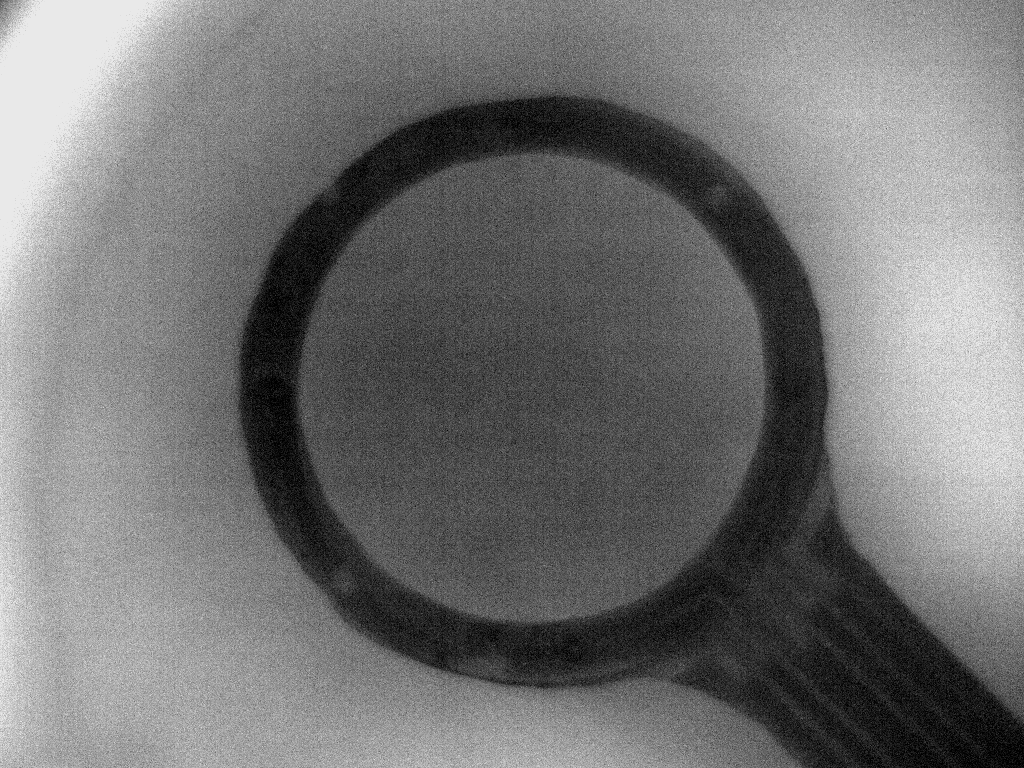
\includegraphics[width=0.39\textwidth,height=0.3\textwidth]{figs/ringplasmglowoben.png}
				\caption{Ein \tilt{frame} ohne Filter für das Licht der Argon-Entladung. Die Helligkeit in der Mitte ist geringer als außerhalb.}
				\label{img:glow}
                \vspace{-0.5cm}
			\end{wrapfigure}

		Im Zuge der Untersuchung einer Quadrupolschwingung bemerkt man leicht, dass die Teilchen des Clusters, zusätzlich zu ihrer Auslenkung in der Ebene, eine bananenartige Bahn mit vertikaler Komponente durchlaufen. Die radiale Anregung dieser Mode enthält jedoch keine solchen Anteile. Diese Beobachtung legt demnach nahe, dass die Randschichtveränderung durch das Einfangpotential nicht vernachlässigbar für die Kinematik des Cluster ist.\\
		Aus den Abschnitten \ref{sub:kaprfplasm} und \ref{sub:rand} wissen wir,  dass sich um elektrische leitfähige Objekte in einem Plasma eine Grenzschicht ausbildet. Weiterhin ist deren Ausdehnung und Eigenschaften abhängig vom Potential des lokalen Plasmas bzw. des Objektes selber. Deswegen ist die Manipulation eines Yukawa-Clusters nicht nur als elektrische Kraft (siehe \ref{img:potential}) durch die Signale der Ring-Segmente zu verstehen, sondern viel mehr als Summe dessen und der Veränderung der lokalen Randschicht, in welcher sich die Staubpartikel befinden.\\
		Ein Maß für ihre Ausdehnung, und somit daraus folgend ihre weiteren Eigenschaften, ist das Leuchten der Neutralgasatome des Argons. Dieses ist intensiver, je größer die vorliegende Elektronendichte ist (siehe \ref{sub:rand}).  Auf Grund dessen erhält man aus einer Intensitätsanalyse des Bereiches aus \ref{img:glow} Informationen über die Stärke der Randschichtveränderungen.\\
        Ohne die, während der restlichen Messungen an den Kameras angebrachten Filter für das Plasmaleuchten, wurden Aufnahmen für Anregungen einer Dipol-, Quadrupol- und Rotationsschwingung gemacht. Bei 200 \tilt{fps} wurden jeweils 2000 \tilt{frames} bei einer Frequenz von 3 und $\unit[10]{Hz}$ gemacht. Von Interesse sind dabei jedoch nur die Bilder der Oberkamera ('grün', siehe \ref{img:glow}). Die \tilt{bitmaps} werden für die Analyse zuerst auf ein \tilt{range of interest} - ein Kreis bzw. eine Kreisscheibe, in welcher das Leuchten ausgewertet werden soll - beschnitten. Anschließend wird das \tilt{ROI} in Radius- und Winkelabschnitte eingeteilt, welche in ihrer Intensität gemittelt werden. Ein anschauliches Beispiel für die Darstellung des Intensitätsverlaufs, in radialer und polarer Auflösung, einer Rotationsschwingung wird in \ref{img:glowanalys} gezeigt.

            \begin{figure}[H]
                    \centering
                    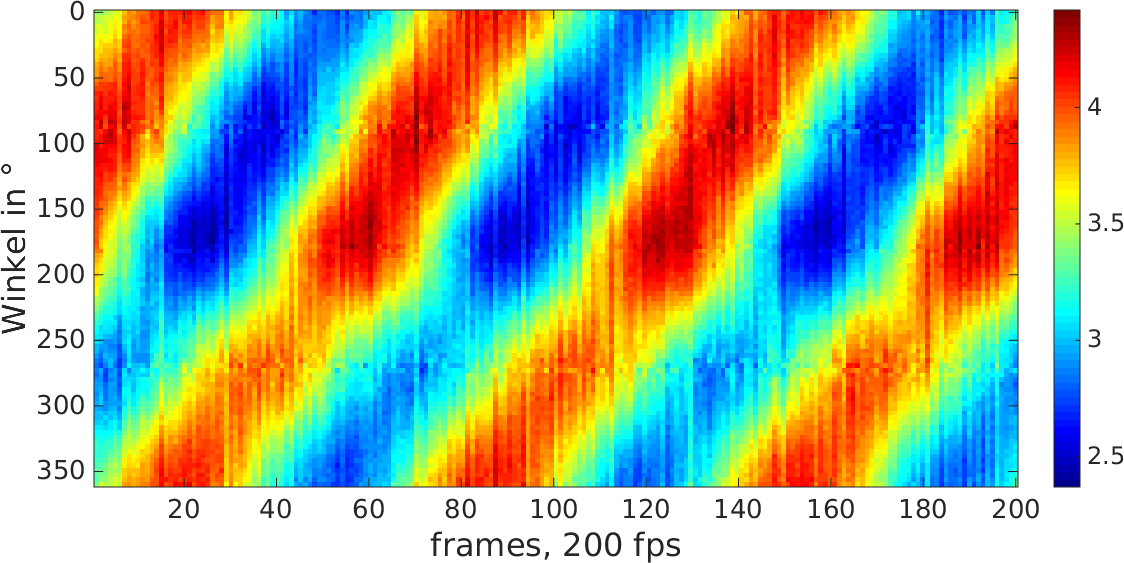
\includegraphics[width=0.8\textwidth,height=0.25\textheight]{figs/glowbeispielrotation3Hzang.png}
            \end{figure}

        \vspace{-0.5cm}

            \begin{figure}[H]
                    \centering
                    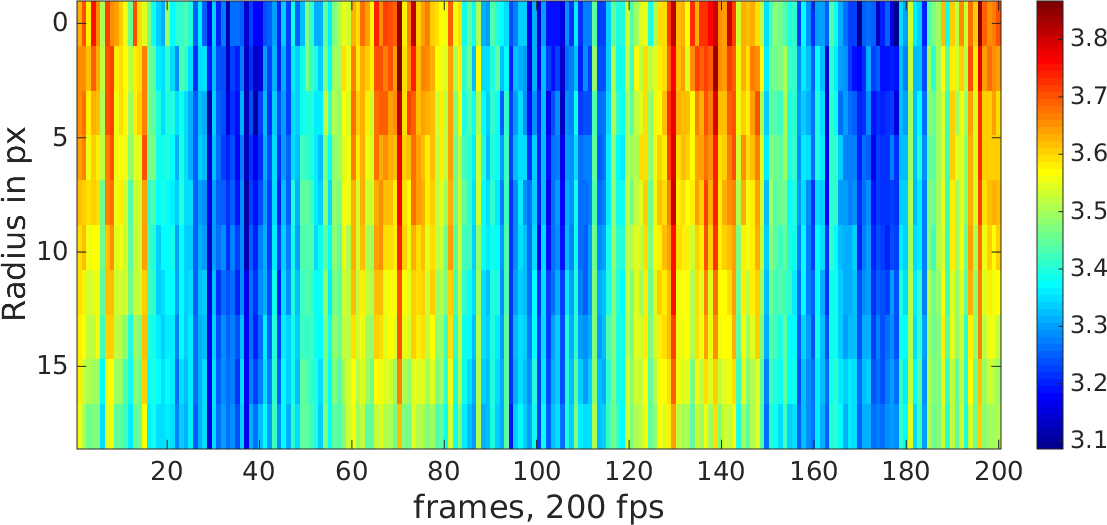
\includegraphics[width=0.8\textwidth,height=0.25\textheight]{figs/glowbeispielrotation3Hzrad.png}
                    \caption{\underline{\fett{oben}}: Winkelaufgelöste Rotationsanregung. Bei $\unit[250]{\degree}$ ist eine Asymmetrie zu erahnen. \underline{\fett{unten}}: Radiale Auflösung. Die Randschichtveränderung ist innen stärker als außen.}
                    \label{img:glowanalys}
            \end{figure}

	\newpage

	\section{Auswertung}\label{sec:auswert}

        \subsection{Untersuchungen der Randschicht}

        \subsection{Elektrische Manipulation}

            \subsubsection{Quadrupol-Anregung}

            \subsubsection{Elektrode mit 6 Segmenten}

         \subsection{Zusammenfassung}

	\newpage

	\section{Literatur}\label{sec:lit}

		\bibliography{all_melzer2.bib}
		\bibliographystyle{unsrt}

	\newpage

	\section{Anhang}\label{sec:anhang}

%		\subsection{Abkürzungsverzeichnis}\label{subsec:abkurz}
%		
%			\begin{acronym}
%				
%			\end{acronym}

\end{document}
